\documentclass[a4paper,12pt]{report}
% es wurde leqno entfernt, da damit die Nummern von Gleichungen links standen
\usepackage{inputenc,fontenc}
\usepackage[a4paper,margin=3cm]{geometry}
\usepackage[english, german]{babel}
\usepackage[ngerman=ngerman]{hyphsubst}
% \usepackage{isodate}
\usepackage[hidelinks]{hyperref}
\usepackage{amsmath, amsfonts, amssymb, amsthm} %% mathematics tools
\usepackage{csquotes}
\usepackage[draft]{listofsymbols}
\usepackage[backend=biber, urldateusetime=true, sorting=none]{biblatex} %% Literature citing engine
\usepackage{subcaption}
\usepackage{graphicx}
\usepackage{algorithm}
\usepackage{algpseudocode}
\usepackage{dsfont} % für charakteristische 1

%%
%% Pflichtangaben -bitte hier einsetzen %%%%%%%%%%%%%%%%%%%%%%%%%%%%%%%%%%%%%%%%%%%%%%
%%
\newcommand{\name}{Göpel}
\newcommand{\vorname}{Noah}
\newcommand{\gebdatum}{01.02.2003}
\newcommand{\ort}{Riesa}
\newcommand{\betreuer}{Prof. Dr. Oliver Sander}
\newcommand{\institut}{Institut für Numerische Mathematik}
\newcommand{\thema}{Gewichtete Eigenwert-Zählung auf einem Intervall}
\newcommand{\datum}{tt.\ mm.\ jjjj} %Format tt.\ mm.\ jjjj

%%%%%%%%%%%%%%%%%%%%%%%%%%%%%%%%%%%%%%%%%%%%%%%%%%%%%%%%%%%%%%%%%%%%%%%%%%%%%%%%%%%%%%


%__________Definitions_____________________________

% Literaturverzeichnis
\addbibresource{Literatur.bib}
\graphicspath{{src/}}

% \newcommand{\bild}[2]{\includegraphics[width=#2\textwidth,height=#2\textheight,keepaspectratio]{#1}}
\newcommand{\bild}[4]{
      \begin{figure}[!htp]
            \centering
            \includegraphics[width=#2\textwidth,height=#2\textheight,keepaspectratio]{#1}
            \caption{#3}
            #4
      \end{figure}
}
\newcommand{\R}{\mathbb R}
\newcommand{\C}{\mathbb C}
\newcommand{\N}{\mathbb N}
\newcommand{\zitat}[1]{\glqq #1\grqq}
\newcommand{\klammer}[1]{\left(#1\right)}
\newcommand{\diag}{\text{diag}}
\newcommand{\rang}{\text{rang}}
\newcommand{\tr}{\text{tr}}
\newcommand{\AlamB}{A-\lambda\,B}
\newcommand{\Cnn}{\C^{n\times n}}
\newcommand{\inv}{^{-1}}
\newcommand{\1}{\mathds{1}}
\newcommand{\Res}{\text{Res}}
\newcommand{\interior}{\text{int}}

% wird für Symbolverzeichnis benutzt, sonst gibt es Fehler
\DeclareOldFontCommand{\bf}{\normalfont\bfseries}{\mathbf}

% Math
\theoremstyle{plain} % text is cursive
\newtheorem{theorem}{Theorem}
\newtheorem{lemma}[theorem]{Lemma}  %% [theorem] means same numbering for theorem and lemma
\newtheorem{proposition}[theorem]{Proposition}
\newtheorem{corollary}[theorem]{Korollar}

\theoremstyle{definition} % text is "upright"
\newtheorem{definition}[theorem]{Definition}
\newtheorem{example}[theorem]{Beispiel}

\theoremstyle{remark}
\newtheorem{remark}[theorem]{Bermerkung}

% diese Befehle werden verwendet, um den Algorithmus 
\floatname{algorithm}{Algorithmus}
\renewcommand{\algorithmicrequire}{\textbf{Eingabe:}}
\renewcommand{\algorithmicensure}{\textbf{Ausgabe:}}

% Symbolverzeichnis
\renewcommand{\symheadingname}{Symbolverzeichnis}
\opensymdef
      % \newsym[]{}{}
      \newsym[Einheitsmatrix]{In}{I_n}
      \newsym[Massenmatrix]{M}{M}
      \newsym[Steifigkeitsmatrix]{K}{K}
      \newsym[Federkraft]{FL}{\overrightarrow{F_L}}
      \newsym[Trägheitskraft]{FT}{\overrightarrow{F_T}}
      \newsym[Auslenkung des k-ten Massepunktes aus der Ruhelage]{xk}{x_k}
      \newsym[Eigenkreisfrequenz]{w}{\omega}
      \newsym[vorgegebenes Intervall]{wAwB}{[\omega_a,\omega_b]}
      \newsym[Eigenwert des Matrix-Pencils, definiert durch $\lambda:=\omega^2$]{lam}{\lambda}
      \newsym[Intervall, definiert durch $\lbrack\lambda_a,\lambda_b\rbrack := \lbrack\omega_a,\omega_b\rbrack$]{lamAlamB}{[\lambda_a,\lambda_b]}
\closesymdef
% , soll zum Schluss frei von Eigenkreisfrequenzen sein

\begin{document}
\selectlanguage{german}

%% Titelseite
\thispagestyle{empty}

\begin{center}
{\Large Technische Universit\"{a}t Dresden\  \ \textbullet\ \ Fakult\"{a}t Mathematik}

\vfil

{\bfseries\Huge\thema}

\vfil
{\LARGE
Bachelorarbeit \\[\bigskipamount]
zur Erlangung des ersten Hochschulgrades\\[\bigskipamount]
\bfseries{\itshape Bachelor of Science  \textup{(}B.Sc.\textup{)}}\\[\bigskipamount]
}

\vfil\vfil

\vfil

vorgelegt von
\\[\bigskipamount]
\textsc{\vorname\ } \MakeUppercase{\name}
\\[\bigskipamount]
(geboren am \gebdatum\ in \textsc{\ort})
\\[\bigskipamount]
Tag der Einreichung: \datum
\\[\bigskipamount]
\betreuer\ (\institut)
\end{center}

\cleardoublepage
%%%%%%%%%%%%%%%%%%%%%%Beginn Ausarbeitung%%%%%%%%%%%%%%%%%%%%%%%%%%%%%%%%
\tableofcontents
\clearpage
\listofsymbols
\clearpage

\chapter{Einleitung}
\label{sec: Einleitung}
      
      Diese Ausarbeitung beschäftigt sich mit numerischen Verfahren, um sicherzustellen, dass für ein gegebenes mechanisches System keine Eigenwerte in einem vorgegebenem festen Intervall liegen.
% hier muss noch einiges getan werden
      Damit kann sichergestellt werden, dass die Eigenfrequenzen des Systems nicht so liegen, dass es zu einer Selbsterregung kommt.

      % Um diese Anforderung zu erfüllen, werden die Eigenwerte des Matrix-Pencils auf diesem Intervall gewichtet gezählt. Man erhält ein Minimierungsproblem,
      % in welchem es gilt, einen Design-Paramerter so anzupassen, dass auf dem Intervall kein Eigenwert des entsprechenden Systems mehr vorhanden ist.
      % Dazu werden in den Kapiteln \ref{sec: MS Matrizen} und \ref{sec: EW Problem} die theoretischen Grundlagen gelegt.
      % Anschließend werden in Kapitel \ref{sec: Quellen} die entscheidende Identität von Futamura und wichtige Überlegungen ausgeführt.

      % Daraufhin werden diese Überlegungen in Kapitel \ref{sec: Programmieren} anhand verschiedener Beispiele implementiert und getestet.

      Die Auswertung und Verbesserung der Implementation folgt in Kapitel \ref{sec: Verbesserungen}.

      % In dieser Ausarbeitung werden die gewichtete Zählung von Eigenwerten auf einem Intervall behandelt, um sicherzustellen,
      % dass bei einem vorgegebenem mechanischem System keine Eigenwerte in einem bestimmten festen Intervall liegen.
      % Dazu wird in den ersten Kapiteln die nötige Theorie anhand der Quellen \cite{grundlageFutamura} und \cite{hauptteilTkachuk} beschrieben.
      % Hier werden Matrix-Pencil und das allgemeinerte Eigenwertproblem verwendet, um 
      % Hierzu nutzt man die Identität von Futamura, um die Zählung der Eigenwerte auf die zugrundeliegenden Matrizen zurückzuführen.


      % und anschließend in Kapitel \ref{sec: Programmieren} in Python angewendet.
      % Daraufhin werden in Kapitel \ref{sec: Verbesserungen} die Ergebnisse kritisch betrachtet und weitere Algorithmen eingeführt, um die Berechnungen zu beschleunigen.
      Zum Schluss werden in Kapitel \ref{sec: Auswertung} die Ergebnisse wiederholt und ein Ausblick in weiterführende Themen gegeben.

      Ferner werden in Kapitel \ref{sec: Verbesserungen} eine Approximation der Matrix-Spur vorgestellt und ebenfalls implementiert.

\chapter{Das allgemeine Eigenwertproblem und die Identität von Futamura}
\label{sec: EW Problem_Futamura}

      Zu Beginn der Ausarbeitung werden einige Resultate über Matrizen und lineare Algebra behandelt.
      Diese werden in Kapitel \ref{sec: EW Zählung} verwendet, um die Zählung der Eigenwerte zu einer differenzierbaren Funktion umzuformen.
      
      \section{Der Matrix-Pencil}
            Betrachte zunächst das Konzept des \zitat{Matrix-Pencils} \cite[S. 32]{matrixPencilDeutsch}, welches in dieser Ausarbeitung eine entscheidende Rolle spielt.
            \begin{definition}(pencil, \cite[S. 375]{matrixGolub})
                  \label{def: pencil}
                  Seien $A$ und $B$ Matrizen in $\C^{n\times n}$, dann wird die Menge aller Matrizen der Form
                  $\AlamB, \lambda \in \C$ Matrix-Pencil genannt.
            \end{definition}

            Laut \cite[S. 375]{matrixGolub} seien die Eigenwerte von $\AlamB$ diejenigen $\lambda \in\C$, für die gelte:
            \begin{equation}
                  \label{eqn: allg EW Problem}
                  (\AlamB)x=0,\quad x\ne 0
            \end{equation}
            
            Hier wird $x\in\C^n$ Eigenvektor genannt.
            Man beachte, dass für $B=\In$ Gleichung (\ref{eqn: allg EW Problem}) die folgende Form annimmt:
            $$(A-\lambda\In)x=0 \Leftrightarrow Ax = \lambda x,$$
            also genau die Form des speziellen Eigenwertproblems.
% gibt es ein Eigenwertproblem und wenn ja, gibt es eine Definition? oder ist es einfach eine Gleichung?
            Daher wird die Suche nach den $\lambda\in\C$, die (\ref{eqn: allg EW Problem}) erfüllen, auch \zitat{allgemeines Eigenwertproblem}\cite[S. 380]{maschinendynamikDresig} genannt, da sie eine allgemeine Form des speziellen Eigenwertproblems darstellen.
            Falls man $\AlamB$ durch die Matrix $C$ ersetzt, so entsteht aus (\ref{eqn: allg EW Problem}) das lineare homogene Gleichungssystem
            $$Cx=0,\quad x\ne 0$$

            Nach einem Resultat aus der linearen Algebra gilt:
% welches Resultat?, ich habe es bis jetzt nur in Skript LA20 gefunden
            $$\det(C)\ne 0 \Leftrightarrow Cx=0 \text{ hat als einzige Lösung }x=0$$
            Durch Negation folgt:
            $$\det(C)=0 \Leftrightarrow \exists x\ne 0: Cx=0$$

            Somit sucht man die Eigenwerte des Matrix-Pencils, in dem man die Nullstellen des Polynoms $\det(\AlamB)$ berechnet\footnote{Man könnte das Polynom $\det(\AlamB)$ als eine Art charakteristisches Polynom des Matrix-Pencils $\AlamB$ betrachten, ähnlich dem charakteristischen Polynom $f(A)$ einer Matrix $A$}.
            
            Daher wird in \cite[S. 375]{matrixGolub} die Menge der Eigenwerte des Matrix-Pencils $\AlamB$ wie folgt definiert:
            \begin{equation}
                  \label{def: EW Pencil}
                  \lambda(A,B):=\{z\in\C:\ \det(A - zB) = 0\}
            \end{equation}

            Laut \cite[S. 375]{matrixGolub} gelte zudem:
            \begin{equation}
                  \label{eqn: n EW äquiv rang B n}
                  \AlamB \text{ hat }n\text{ Eigenwerte}\Leftrightarrow \rang(B)=n
            \end{equation}
            Dieses Resultat wird für Kapitel \ref{sec: EW Zählung} relevant werden und kann mithilfe von Theorem \ref{thrm: allg Schur Zerlegung} gezeigt werden.

            Man benötigt für die Identität von Futamura aus Kapitel \ref{sec: Futamura} zudem eine weitere Definition:
            \begin{definition}(Regulärer Matrix-Pencil, vgl. \cite[S. 784]{regularMatrixPencil})\\
                  \label{def: regulärer Pencil}
                  Ein Matrix-Pencil $A+\lambda B$ wird regulär genannt, wenn $A,B\in \Cnn$ und
                  $$\det(A+\lambda B)\ne 0$$ 
            \end{definition}

            Beachte, dass hier zwar der Matrix-Pencil mit $+$ statt $-$ angegeben wurde, aber diese Definitionen sind gleichwertig, da man $\tilde \lambda := -\lambda$ in den Matrix-Pencil einsetzen kann.
            \begin{remark}
                  \label{bem: B reg impl pencil reg}
                  Diese Definition bedeutet insbesondere, dass der Matrix-Pencil regulär ist, falls B regulär ist, denn es gilt:
                  \begin{align*}
                        B\text{ regulär} \Leftrightarrow & \rang(B)=n\Leftrightarrow |\lambda(A,B)| = n<\infty\\
                        \Rightarrow & \exists z\in\C\setminus\lambda(A,B): \det(A+zB) \ne 0 \Leftrightarrow \AlamB \text{ regulär}
                  \end{align*}
                  Wobei (\ref{eqn: n EW äquiv rang B n}) und die Überabzählbarkeit von $\C$ verwendet wurde.
            \end{remark}
            
% man kann auch noch Korollar 2.3.11 (LinAlg Werner, S. 50) ansprechen

      \section{Die Schur-Zerlegung}
            In diesem Kapitel werden weitere wichtige Konzepte vorgestellt, die für Kapitel \ref{sec: Futamura} benötigt werden.

            \begin{definition}(\cite[S. 73]{matrixGolub})
                  Sei $Q \in\C^{n\times n}$, dann wird $Q$ unitär genannt, wenn
                  $$Q^HQ = QQ^H=\In$$
            \end{definition}

            Hier ist $Q^H$ die Adjungierte von $Q$, also die Matrix, die durch komplexe Konjugation und Transponierung von $Q$ entsteht, siehe auch \cite[S. 14]{matrixGolub}.

%             \begin{theorem}(vgl. Theorem 7.1.3 (Schur Decomposition)\cite[S. 313]{matrixGolub})\\
%                   \label{thrm: Schur Zerlegung}
%                   Wenn $A \in \C^{n\times n}$, dann existiert eine unitäre Matrix $Q\in\C^{n\times n}$, sodass
%                   \begin{equation}
%                         \label{eqn: Schur_Resultat}
%                         Q^H\,AQ = T = D+N
%                   \end{equation}
%                   mit $D=\diag(\lambda_1,\dots,\lambda_n)$ und $N\in\C^{n\times n}$ strikter oberer Dreiecksmatrix.
%                   Ferner kann $Q$ so gewählt werden, dass die Eigenwerte $\lambda_i$ in beliebiger Reihenfolge auf der Diagonalen auftauchen.
%             \end{theorem}

%             Um dieses Theorem zu beweisen, benötigt man ein Hilfslemma aus \cite[S.312]{matrixGolub}.
%             Das folgende Resultat wird einfachheitshalber in dem speziellen Fall vorgestellt, wie es für den Beweis von Theorem \ref{thrm: Schur Zerlegung} benötigt wird.

%             \begin{lemma}(vgl. Lemma 7.1.2\cite[S. 312]{matrixGolub})
%                   \label{lemma: Hilfe Schur}\\
%                   Falls ein $A\in\C^{n\times n}, \lambda\in \C$ Eigenwert von $A$ und $X\in \C^{n}$
%                   \begin{equation}
%                         \label{eqn: Hilfslemma Schur_Bed}
%                         AX = X\lambda,\qquad \rang(X)=1
%                   \end{equation}
                  
%                   erfüllen, dann existiert ein $Q\in \C^{n\times n}$ unitär, sodass
%                   $$Q^H\,AQ = T =  \begin{bmatrix}
%                         \lambda & T_{12} \\
%                         0 & T_{22} \\
%                         \end{bmatrix}$$
%                   mit $T_{22}\in \C^{(n-1)\times(n-1)}$
%             \end{lemma}

%             Beweis:
%             Erhalte mit \cite[S. 233]{matrixGolub} eine komplexe QR-Zerlegung für $X$. Es gilt dann
%             $$X = Q\,R$$
%             mit $Q\in \C^{n \times n}$ unitär und $R = [r,0,\dots,0]^\top\in \C^n$.
%             Durch Einsetzen in (\ref{eqn: Hilfslemma Schur_Bed}) und Multiplikation mit $Q^H$ folgt
%             \begin{equation}
%                   \label{eqn: Hilfslemma_Schur_Gl}
%                   \underbrace{Q^H\,AQ}_{=:T}\ R = Q^H\,Q\ R\ \lambda
%             \end{equation}
% % man könnte hier R statt dem Vektor nutzen, dann wäre es kompakter
%             hier ist noch $T:=\begin{matrix}
%                   \begin{bmatrix}
%                         T_{11} & T_{12}\\
%                         T_{21} & T_{22}\\
%                   \end{bmatrix} & \begin{matrix}
%                   \text{\small 1} \\\text{\small{n-1}}
%                   \end{matrix} \\
%                   \begin{matrix}
%                   \text{\small 1} &  \text{  \small{n-1}}\\
%                   \end{matrix} &  \\
%                   \end{matrix}$\\

%             Durch Ausmultiplizieren von (\ref{eqn: Hilfslemma_Schur_Gl}) folgen die Gleichungen\\

%             $$\begin{aligned}
%                   T_{11}\,r =& r\,\lambda\\
%                   T_{21}\,r =& 0
%             \end{aligned}$$

%             und mit $\rang(X)=1 \Rightarrow X\ne 0 \Rightarrow r\ne 0$ folgt $T_{11} = \lambda,\ T_{21} = 0$.\qed

%             Nach \cite[S. 312]{matrixGolub} gelte ferner $\lambda(A) = \lambda(T) = \{\lambda\}\cup\lambda(T_{22})$.\\
            

%             Nun können wir Theorem \ref{thrm: Schur Zerlegung} beweisen.

%             Beweis Theorem \ref{thrm: Schur Zerlegung} (vgl. \cite[S. 313]{matrixGolub}):

%             Offenbar gilt für $n=1$:\\
%             $A$ ist ein Skalar, wodurch (\ref{eqn: Schur_Resultat}) für alle $Q$ unitär erfüllt ist.\\
%             Sei nun $n>1$ und (\ref{eqn: Schur_Resultat}) gelte für alle $k<n$, dann gilt für einen beliebigen Eigenwert $\lambda$ von $A$ und zugehörigen Eigenvektor $X$:
%             $$AX = \lambda X = X \lambda,\quad X\in \C^n, X\ne 0$$
%             Nach Lemma \ref{lemma: Hilfe Schur} existiert $U\in \C^{n\times n}$ unitär, sodass
%             $$U^H\, AU = \begin{bmatrix}
%                   \lambda & T_{12} \\
%                   0 & T_{22} \\
%                   \end{bmatrix}$$
%             Da aber $T_{22}\in\C^{(n-1)\times(n-1)}$, so gilt nach der Induktionsvoraussetzung:
%             $$\widetilde U^H\,T_{22}\widetilde U = R,$$
%             wobei $R\in\C^{(n-1)\times(n-1)}$  rechte obere Dreiecksmatrix, $\widetilde U \in\C^{(n-1)\times(n-1)}$ unitär.

%             Sei nun $Q:=U\cdot\begin{bmatrix}
%                   1&0\\
%                   0&\widetilde U
%             \end{bmatrix}$

%             dann gilt mit\footnote{die folgende Gleichung stammt aus \cite{conjugateTranspose}, Beweis ebenfalls dort zu finden}
% % Fussnote vielleicht scheisse platziert
%             \begin{equation}
%                   \label{eqn: Produkt Adjungierter}
%                   \klammer{AB}^H = B^HA^H,\quad A,B\in \C^{n\times n}
%             \end{equation}
%             für (\ref{eqn: Schur_Resultat}):
%             $$\begin{aligned}
%                   Q^H\,AQ =& \begin{bmatrix}
%                         1&0\\
%                         0&\widetilde U
%                   \end{bmatrix}^H\,U^H\,AU \begin{bmatrix}
%                         1&0\\
%                         0&\widetilde U
%                   \end{bmatrix} = \begin{bmatrix}
%                         1&0\\
%                         0&\widetilde U^H
%                   \end{bmatrix}
%                   \begin{bmatrix}
%                         \lambda & T_{12} \\
%                         0 & T_{22} \\
%                   \end{bmatrix}
%                   \begin{bmatrix}
%                         1&0\\
%                         0&\widetilde U
%                   \end{bmatrix}\\
%                   =& \begin{bmatrix}
%                         \lambda&T_{12}\\
%                         0&\widetilde U^H\, T_{22}
%                   \end{bmatrix}
%                   \begin{bmatrix}
%                         1&0\\
%                         0&\widetilde U
%                   \end{bmatrix}
%                   = \begin{bmatrix}
%                         \lambda&T_{12}\,\widetilde U\\
%                         0&\widetilde U^H\, T_{22}\, \widetilde U
%                   \end{bmatrix}\\
%                   =& \begin{bmatrix}
%                         \lambda&T_{12}\,\widetilde U\\
%                         0&R
%                   \end{bmatrix}
%             \end{aligned}$$
%             Wobei verwendet wurde, dass nach Definition die komplex Konjugation skalar angewendet wird\footnote{siehe \cite[S. 14]{matrixGolub}}, also es gilt:
           
%             \begin{equation}
%             \label{eqn: Adjungierte reinziehen}
%                   \begin{bmatrix}
%                         1&0\\
%                         0&\widetilde U
%                   \end{bmatrix}^H = \overline{\begin{bmatrix}
%                         1&0\\
%                         0&\widetilde U^T
%                   \end{bmatrix}} = \begin{bmatrix}
%                         \overline{1}&0\\
%                         0&\overline{\widetilde U^T}
%                   \end{bmatrix} = \begin{bmatrix}
%                         1&0\\
%                         0&\widetilde U^H
%                   \end{bmatrix}
%             \end{equation}

%             Damit ist gezeigt, dass $Q^H\,AQ$ eine rechte obere Dreiecksmatrix ist.

%             $D = \diag(\lambda_1,\dots,\lambda_n)$ folgt mit Korollar 4.2.3 aus \cite[S. 80]{LinAlgWerner}.
%             Die Beliebigkeit der Anordnung der Eigenwerte auf der Diagonalen erhält man durch rekursives Anwenden von Theorem \ref{thrm: Schur Zerlegung} auf die Matrix $T_{22}$.
%             Es fehlt noch zu zeigen, dass $Q$ unitär ist, was aber mit (\ref{eqn: Produkt Adjungierter}) und (\ref{eqn: Adjungierte reinziehen}) einfach gezeigt werden kann. \qed\\

            Mithilfe dieser Definition kann nun die allgemeine Schur-Zerlegung vorgestellt werden.
            Diese wird für den Beweis der Identität von Futamura in Kapitel \ref{sec: Futamura} benötigt.
%hier kann noch viel mehr erzählt werden: die Eigenschaft der Eigenwerte ist von entscheidender Relevanz
            \begin{theorem}(Generalized Schur Decompositon, \cite[S. 377]{matrixGolub})
                  \label{thrm: allg Schur Zerlegung}
                  Seien $A, B \in \C^{n\times n}$, dann existieren $Q$ und $Z$ unitär, sodass
                  \begin{equation}
                        \label{eqn: allg Schur_Resultat}
                        Q^H\,AZ = T,\quad Q^H\, BZ = S
                  \end{equation}
                  mit $T$ und $S$ obere Dreiecksmatrizen.
                  Falls für ein $k\in \{1,\dots, n\}\ t_{kk}=s_{kk}=0$, dann gilt $\lambda(A, B) = \C$, sonst
                  \begin{equation}
                        \label{eqn: EW Pencil nach Schur}
                        \lambda(A, B) = \{t_{ii}/s_{ii}:\, s_{ii}\ne 0\}
                  \end{equation}
            \end{theorem}
            Beweis: siehe \cite[S. 377]{matrixGolub}\qed
      
      \section{Die Identität von Futamura}
      \label{sec: Futamura}

            Nach den Vorbereitungen, die in vorherigen Abschnitten gemacht wurden, kann nun die Identität von Futamura beschrieben und gezeigt werden.

            Das folgende Theorem wird für das Finden einer Zielfunktion von entscheidender Relevanz sein,
            da durch diese Aussage in Kapitel \ref{sec: EW Zählung} ein Zusammenhang zwischen der Anzahl der Eigenwerte auf einem Intervall und einem Kurvenintegral über Matrizen gezeigt werden kann.

            \begin{theorem}(vgl. \cite[S. 127]{grundlageFutamura})
                  \label{thrm: IdentitätFutamura}\\
                  Seien $A, B\in\Cnn, z\in \C$, sodass $(zB-A)$ ein regulärer Matrix-Pencil ist, dann gibt es unitäre Matrizen $Q$ und $U \in\Cnn$, sodass
                  $$A = QTU^H,\quad B=QSU^H$$
                  und
                  \begin{equation}
                        \label{eqn: Resultat_Futamura}
                        \tr((zB-A)\inv B) = \sum_{j\in N}\frac{1}{z-\lambda_j},
                  \end{equation}
                  gilt, wobei $N:=\{i\in\{1,\dots,n\}: s_{ii}\ne 0\}$ und $\lambda_j$ die Eigenwerte des Matrix-Pencils sind.
                  $S$ und $T$ sind hier obere Dreiecksmatrizen.
            \end{theorem}
% warum zB-A? für Eigenwerte macht es keinen Unterschied
            Beweis:
            Nach Theorem \ref{thrm: allg Schur Zerlegung} gibt es unitäre Matrizen $Q$ und $U\in\Cnn$, sodass nach entsprechender Multiplikation gilt:
            $$A=QTU^H,\quad B=QSU^H$$
            mit $T,S\in\Cnn$ obere Dreiecksmatrizen.
            
            Hierbei sind $S$ und $T$ obere Dreiecksmatrizen, und es gilt:
            $$\lambda(B)=\lambda(S) = \{s_{ii}:i=1,\dots,n\},$$
            aber diese Eigenwerte sind noch ungeordnet und man kann nicht wie in \cite{grundlageFutamura}:
            \begin{align*}
                  s_{ii} = \begin{cases}
                        \ne 0 & : i\le n'\\
                        0 & : i>n'
                  \end{cases}
            \end{align*}
            annehmen für $n':=|\{i\in\{1,\dots,n\}: s_{ii}\ne 0\}|$.

            Mithilfe der Definition
            $$N:=\{i=1,\dots,n: s_{ii}\ne 0\}$$
            kann dies aber umgangen werden.

            Man kann folgern:
            \begin{align*}
                  (zB-A)\inv B =& (z\,QSU^H-QTU^H)\inv QSU^H = (Q(zS-T)U^H)\inv QSU^H \\
                  =& U(zS-T)\inv Q^H\,QSU^H = U(zS-T)\inv S\,U\inv
            \end{align*}

            Man sieht, dass $(zB-A)\inv B$ und  $(zS-T)\inv S$ ähnlich zueinander sind.\\
            Da die Spur invariant unter Ähnlichkeitstransformation ist\footnote{vgl. 3. Exercise unter Example 1.3.5 in \cite{matrixSpur}}, gilt
            \begin{equation}
                  \label{eqn: Haltepunkt Bew Futamura}
                  \tr((zB-A)\inv B) = \tr((zS-T)\inv S) = \sum_{i=1}^{n}((zS-T)\inv S)_{ii}
            \end{equation}

            Für die folgenden Beweisschritte benötigt man einige Aussagen über obere Dreiecksmatrizen, hierbei ist mit $X_{ij}$ der Eintag von X in Zeile $i$ und Spalte $j$ gemeint.

            \begin{lemma}
                  \label{Hilfslemma_Futamura: Inv Dreieck}
                  Die Inverse einer oberen Dreiecksmatrix $A$ ist eine obere Dreiecksmatrix
            \end{lemma}
            Beweis: Anwenden des Gauß-Jordan-Algorithmus zur Bestimmung der Inversen auf $(A|\In)$ mit $A$ rechte obere Dreiecksmatrix\qed
% man könnte auch mit Gramerschen Regel argumentieren, aber da ist es schwer zu beweisen, dass die Kofaktoren null sind
% hier gibt es noch Verbesserungsbedarf

            \begin{lemma}
                  \label{Hilfslemma_Futamura: Prod Dreieck}
                  Seien X und Y obere Dreiecksmatrizen, dann gilt:
                  $$(XY)_{ii} = X_{ii}\, Y_{ii}$$
            \end{lemma}
            Beweis:
            $$(XY)_{ii} = \sum_{k=1}^n X_{ik}Y_{ki} = \sum_{k=I}^{n}X_{ik}Y_{ki} = \sum_{k=I}^{i}X_{ik}Y_{ki} = X_{ii} Y_{ii}$$
            wobei verwendet wurde, dass für eine obere Dreiecksmatrix $A$ nach Definition gilt:
            $A_{ij} = 0 \text{ für }i>j$\qed

            \begin{lemma}
                  \label{Hilfslemma_Futamura: Diag Inv Dreieck}
                  Für eine invertierbare obere Dreiecksmatrix X gilt:
                  $$(X\inv)_{ii} = \frac 1 {(X)_{ii}}$$
            \end{lemma}
            Beweis: Sei $i\in\{1,\dots,n\}$ fest, dann gilt
            $$\In = X\,X\inv \Rightarrow 1 = X_{ii}(X\inv)_{ii} \Rightarrow (X\inv)_{ii} = \frac 1 {(X)_{ii}}$$
            Hier wurde Lemma \ref{Hilfslemma_Futamura: Prod Dreieck} und
            $$X \text{ invertierbar}\Rightarrow \det X = \prod_{k=1}^{n}X_{kk}\ne 0\Rightarrow X_{kk}\ne 0\quad \forall k=1,\dots,n$$
            verwendet.\qed\\

            Nun kann man den Beweis für Theorem \ref{thrm: IdentitätFutamura} vervollständigen:
            Mit den Lemmata \ref{Hilfslemma_Futamura: Inv Dreieck}, \ref{Hilfslemma_Futamura: Prod Dreieck} und \ref{Hilfslemma_Futamura: Diag Inv Dreieck} folgt für (\ref{eqn: Haltepunkt Bew Futamura}):
            \begin{align*}
                  \tr((zB-A)\inv B) =& \sum_{i=1}^{n}((zS-T)\inv)_{ii}\ S_{ii} = \sum_{i=1}^{n}((zS-T)_{ii})\inv\ S_{ii}\\
                  =& \sum_{i=1}^{n}\frac{s_{ii}}{z\,s_{ii}-t_{ii}} = \sum_{i\in N}\frac{s_{ii}}{s_{ii}(z-t_{ii}\, s_{ii}\inv)}\\
                  =& \sum_{i\in N} \frac{1}{z-\lambda_i}
            \end{align*}

            mit
            $$\lambda_i = \frac{t_{ii}}{s_{ii}},\quad i\in N.$$

            Nach Theorem \ref{thrm: allg Schur Zerlegung} und der Definition von $N$ gilt:

            $$\lambda(A, B) = \left\{\frac{t_{ii}}{s_{ii}} : s_{ii}\ne 0\right\} = \{\lambda_i: i\in N\}$$
            somit sind die Eigenwerte des Matrix-Pencils genau die Polstellen der Funktion $\tr((zB-A)\inv B)$.

            In Kapitel \ref{sec: EW Zählung} wird daher das Residuentheorem auf ein Kurvenintegral\\
            über $\tr((zB-A)\inv B)$ angewendet, um die Anzahl der Eigenwerte zu bestimmen.
            Genau dies ist auch die Grundidee in \cite{grundlageFutamura,hauptteilTkachuk}.
% hier noch entscheiden, was drin gelassen wird
            
\chapter{Massen- und Steifigkeitsmatrizen}
\label{sec: MS Matrizen}
      Die Berechnung von Eigenkreisfrequenzen hat in der Mechanik einen besonderen Stand:
      Durch die Betrachtung von Systemen und der Berechnung von Eigenfrequenzen, kann vorhergesagt werden, mit welchen Frequenzen das System schwingen wird.

      Durch das kontrollierte Verändern eines Design-Parameters $s$ kann sichergestellt werden, dass keine Eigenfrequenz des Systems in einem vorgegebenen Intervall liegt.
      Durch die Eliminierung von allen Eigenwerten aus diesem Intervall wird garantiert, dass keine Frequenz in diesem Intervall das System anregt.
      Es kommt daher zu keiner Interferenz und Überlagerung, was für große mechanische Systeme katastrophal sein kann.

      In dieser Ausarbeitung werden die folgenden Systeme untersucht:
      \begin{figure}[ht]
            \centering
            \begin{minipage}[ht]{0.49\linewidth}
                  \centering
                  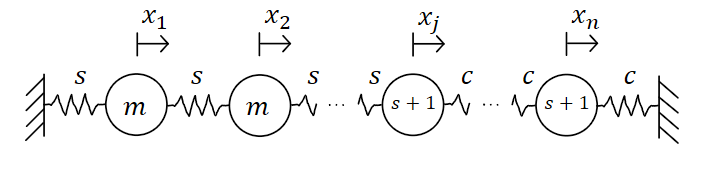
\includegraphics[width=0.9\textwidth, keepaspectratio]{./System1.png}
                  \caption{System 1}
                  \label{fig: System 1}
            \end{minipage}
            \hfill
            \begin{minipage}[ht]{0.49\linewidth}
                  \centering
                  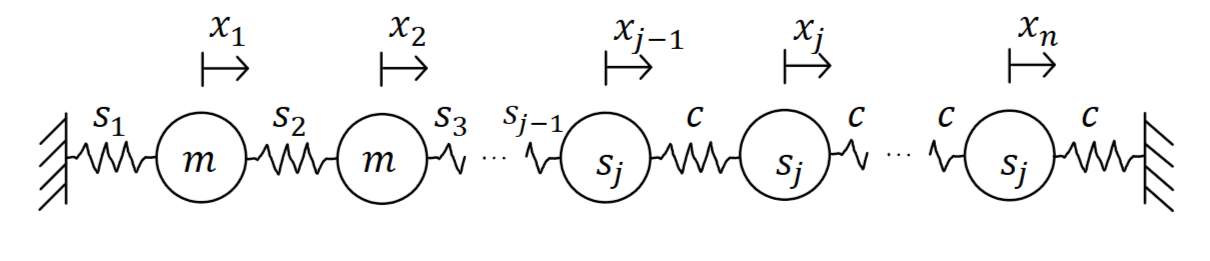
\includegraphics[width=0.9\textwidth, keepaspectratio]{./System2.png}
                  \caption{System 2}
                  \label{fig: System 2}
            \end{minipage}
      \end{figure}

      Der Vektor $x = (x_1,\dots,x_n)^T$ enthält hier die Auslenkungen der Massen aus ihrer Ruhelage und $s\in\R^l$ wird Design-Parameter (vgl. \cite[S. 2]{hauptteilTkachuk}) genannt, da die Eigenschaften des Systems, wie die Eigenkreisfrequenzen, von ihm abhängen.

      Die Systeme aus Abb. \ref{fig: System 1} und \ref{fig: System 2} werden \zitat{Schwingerketten}\cite[S. 236]{maschinendynamikDresig} genannt, da sie aus starren Massen und masselosen Federn bestehen, die linear miteinander verbunden sind.
      Es existieren zudem in diesen Systemen keine Dämpfung.
      
      Laut \cite[S. 362-365]{maschinendynamikDresig} könne man für diese Systeme die \zitat{Differentialgleichung der freien Schwingungen}\cite[S. 365]{maschinendynamikDresig} erhalten, wenn man für jede Masse ein Kräftegleichgewicht aufstellt.
      Diese Differentialgleichung besitzt folgende Form:
      \begin{equation}
            \label{eqn: Dgl freie Schwingungen}
            Kx+M\ddot x = 0
      \end{equation}

      wobei $K$ die Steifigkeitsmatrix und $M$ die Massenmatrix des Systems sind.
% bin ich genug auf d
      Da genau diese Matrizen benötigt werden, um die Eigenkreisfrequenzen zu berechnen, ist das Ziel dieses Kapitels die Systeme von Kräftegleichgewichten aufzustellen und anschließend so umzuformen, dass eine Gleichung der Form (\ref{eqn: Dgl freie Schwingungen}) entsteht.
      Anhand dieser Gleichung werden die Matrizen abgelesen.

      Dafür wird der erste Abschnitt die im System wirkenden Kräfte und die Anwendung des Prinzips von d'Alembert behandeln.
      Im zweiten Abschnitt werden die Matrizen der Systeme bestimmt und anschließend wird in Abschnitt \ref{sec: Formel EW} die Formel für die Berechnung der Eigenkreisfrequenzen hergeleitet. 
      
      \section{Herleitung durch das Prinzip von d'Alembert}
            Nach \cite{d_AlembertPrinzip} besage das Prinzip von d'Alembert, dass die Summe aller wirkenden Kräfte in einem beschleunigten System verschwinde.

            Somit wird zuerst ein Kräftegleichgewicht aufgestellt und anschließend in eine Gleichung über Matrizen umgeformt, wodurch man die Massen- und Steifigkeitsmatrix erhält.
% In Maschinendynamik war von Koeffizientenvgl die Rede, könnte man auch einbauen
% Es muss irgendwo eine Quelle geben, die genau das sagt
            Da diese Herleitung auf Kräftegleichgewichten beruht, werden nun die agierenden Kräfte kurz erläutert:

            Die Federkraft \FL wird laut \cite{federkraft} durch
            \begin{equation}
                  \label{eqn: Federkraft}
                  \FL = -c\cdot s
            \end{equation}
            berechnet, wobei $c$ die Federkonstante und $s$ die Auslenkung der Feder aus der Ruhelage ist.

            Beachte, dass die Kraft entgegen der Auslenkung wirkt, da bei Auslenkung die Feder in die Ruhelage zurückkehren will.
% Quelle finden
                  
            Die Trägheitskraft \FT ist nach \cite{trägheitskraft} definiert durch:
            \begin{equation}
                  \label{eqn: Trägheitskraft}
                  \FT = -m\cdot a
            \end{equation}
            mit Masse $m$ und Beschleunigungsvektor $a$.    
            
            Auch hier wirkt die Kraft wieder der Beschleunigung entgegen.

            Um das Schemas der Kräfte klarer zu gestalten, werden die Kraftpfeile immer in die der Auslengung entgegengesetzte Richtung gezeichnet und die Minuszeichen weggelassen,
            somit werden in den Kraftschemas keine negativen Beträge verwendet.
% Schemas, Kraftschemas,...
            Beide Kräfte werden in Abb. \ref{fig: KräfteAnFeder} veranschaulicht.

            \bild{Federkraft und Trägheitskraft.png}{0.3}{wirkende Kräfte an Masse mit Feder}{\label{fig: KräfteAnFeder}}

            In Abb. \ref{fig: KräfteAnFeder} ist $z$ die Auslenkung und demnach gilt $F_L = c\cdot z$ (vgl. \cite{federkraft}).

            Da in dieser Ausarbeitung nur Feder-Masse-Systeme behandelt werden, kann man $s$ und $a$ auf die Auslenkungen $(\xk)_k$ zurückführen:
            Im Allgemeinen wird hier $s$ durch $(x_{k+1}-\xk)$ und $a$, wie schon in Abb. \ref{fig: KräfteAnFeder}, durch die zweite Ableitung $\ddot \xk$ ersetzt.
% Man könnte es auch umschreiben
            Betrachte nun ein System mit 3 Massen, wie es in Abb. \ref{fig: 3 Massen System} dargestellt wird.
            Anhand dieses Systems soll eine allgemeines Kräftegleichgewicht aufgestellt werden.

            \begin{figure}[ht]
                  \centering
                  \begin{minipage}[ht]{0.49\linewidth}
                        \centering
                        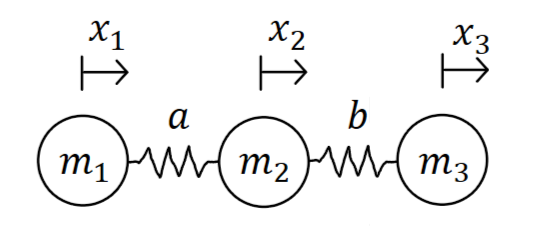
\includegraphics[width=0.7\textwidth, keepaspectratio]{./src/3 Massen System.png}
                        \caption{System mit 3 Massen}
                        \label{fig: 3 Massen System}
                  \end{minipage}
                  \hfill
                  \begin{minipage}[ht]{0.49\linewidth}
                        \centering
                        \includegraphics[width=0.7\textwidth, keepaspectratio]{./src/Kräfte Masse 1D.png}
                        \caption{Kräfte an frei geschnittener Masse}
                        \label{fig: Kräfte Masse 1D}
                  \end{minipage}
            \end{figure}

            Für $m_2$ erhält man die wirkenden Kräfte, wie sie in Abb. \ref{fig: Kräfte Masse 1D} dargestellt wurden.

            Mit dem Prinzip von d'Alembert führt dies auf die Gleichung
            \begin{equation}
                  \label{eqn: Gl für Masse}
                  m_2\,\ddot x_2 + a\,(x_2-x_1) - b\,(x_3-x_2) = 0
            \end{equation}

            Nehme man an, man hat Dirichlet-Randbedingungen, also es gelte zum Beispiel $x_1 \equiv 0$, dann würde man aus (\ref{eqn: Gl für Masse})

            \begin{equation}
                  \label{eqn: Gl für Masse mit Rand links}
                  m_2\,\ddot x_2 + a\,x_2 - b\,(x_3-x_2) = m_2\,\ddot x_2 + (a+b)\,x_2 -b\,x_3 = 0
            \end{equation}
            erhalten.

            In (\ref{eqn: Gl für Masse mit Rand links}) kann die erste Masse als Rand betrachtet werden.
            Eine Gleichung dieser Form wird daher in den Systemen aus Abb. \ref{fig: System 1} und \ref{fig: System 2} für die linken Massen gelten.

      \section{Ermittlung der Matrizen der Modellprobleme}
            Berechne nun die Matrizen der Systeme.
            Während die Systeme der Gleichungen allgemein gehalten werden, verwende für die endgültige Definition der Matrizen $K$ und $M$
            \begin{equation}
                  \label{def: nUndJ explizit}
                  n=8, j=n/2
            \end{equation}
            Beginne dazu mit dem System aus Abb. \ref{fig: System 1}.

            Die Form der Gleichung für die linke Masse ist durch (\ref{eqn: Gl für Masse mit Rand links}) gegeben.
            Für $k=2,\dots, n-1$ gilt eine Gleichung der Form (\ref{eqn: Gl für Masse}).
            
            Da die letzte Masse durch die rechte Feder mit dem Rand verbunden ist, gilt also $x_{n+1} \equiv 0$.
            Und analog zu (\ref{eqn: Gl für Masse mit Rand links}) erhält man
            $$(s+1)\,\ddot x_n + c\,(x_n-x_{n-1}) + c\,x_n = 0.$$  

            Falls man nun alle Massen, Federkonstanten und Auslenkungen einsetzt, so erhält man nach Umstellen das Gleichungssystem

            $$\begin{cases}
                  m\ \ddot x_1 + 2s\,x_1 - s\,x_2 & = 0   \\
                  m\,\ddot x_k -s\,x_{k-1} + 2s\,x_k -s\,x_{k+1} & = 0,\quad k=2,\dots,j-1\\
                  (s+1)\,\ddot x_j -s\,x_{j-1} + (s+c)\,x_j -c\,x_{j+1} & = 0\\
                  (s+1)\,\ddot x_k -c\,x_{k-1} + 2c\,x_k -c\,x_{k+1} & = 0,\quad k=j+1,\dots,n-1\\
                  (s+1)\,\ddot x_n -c\,x_{n-1}+ 2c\,x_n & = 0
            \end{cases}$$

            Dieses System kann man zusammenfassen zu der Gleichung (\ref{eqn: Dgl freie Schwingungen}),
            wobei
            \begin{align}
                  M &= \diag(m, m, m, s+1, s+1,s+1, s+1,  s+1),\label{def: M1}\\
                  K &= \begin{pmatrix}
                        2s & -s &  &  &  &  &  &  \\
                        -s &  2s& -s &  &  &  &0  &  \\
                         & -s & 2s & -s &  &  &  &  \\
                         &  & -s & s+c & -c &  &  &  \\
                         &  &  & -c & 2c & -c &  &  \\
                         &  &  &  & -c & 2c & -c &  \\
                         & 0 &  &  &  & -c & 2c &  -c\\
                         &  &  &  &  &  & -c & 2c \\
                        \end{pmatrix}\label{def: K1}
            \end{align}\\

            Wende dieses Vorgehen auch für das System aus Abb. \ref{fig: System 2} an und erhalte
            
            $$\begin{cases}
                  m\ \ddot x_1 + (s_1+s_2)\,x_1 - s_2\,x_2 & = 0   \\
                  m\,\ddot x_k -s_k\,x_{k-1} + (s_k+s_{k+1})\,x_k -s_{k+1}\,x_{k+1} & = 0,\quad k=2,\dots,j-2\\
                  s_j\,\ddot x_{j-1} -s_{j-1}\,x_{j-2} + (s_{j-1}+c)\,x_{j-1} -c\,x_{j+1} & = 0\\
                  s_j\,\ddot x_k -c\,x_{k-1} + 2c\,x_k -c\,x_{k+1} & = 0,\quad k=j,\dots,n-1\\
                  s_j\,\ddot x_n -c\,x_{n-1}+ 2c\,x_n & = 0
            \end{cases}$$
            

            Dieses System kann man analog zu oben zu der Gleichung (\ref{eqn: Dgl freie Schwingungen}) umformen.
            Hier gilt nun aber
            \begin{align}
                  M &= \diag(m, m, s_4, s_4, s_4, s_4, s_4, s_4)\label{def: M2}\\
                  K &= \begin{pmatrix}
                        s_1+s_2 & -s_2 &  &  &  &  &  &  \\
                        -s_2 &  s_2+s_3& -s_3 &  &  &  &0  &  \\
                              & -s_3 & s_3+c & -c &  &  &  &  \\
                              &  & -c & 2c & -c &  &  &  \\
                              &  &  & -c & 2c & -c &  &  \\
                              &  &  &  & -c & 2c & -c &  \\
                              & 0 & &  &  & -c & 2c &  -c\\
                              &  &  &  &  &  & -c & 2c \\
                        \end{pmatrix}\label{def: K2}
            \end{align}
                  
% hier muss was über die Eigenschaften gesagt werden

      \section{Zusammenhang Eigenwert und Eigenfrequenz}
            \label{sec: Formel EW}      
            Nach der Ermittlung der zugehörigen Matrizen bestimme nun die Formel für die Eigenkreisfrequenzen eines Systems.

            Die Schritte in diesem Abschnitt folgen \cite[S. 380]{maschinendynamikDresig} und \cite[S. 2]{hauptteilTkachuk}.
            Nach \cite[S. 380]{maschinendynamikDresig} gelte für die Auslenkungen der Massen mit $x$ statt $q$:
            $$x(t) = v\,\exp(i\w t),\ \ \ddot x(t) = -\w^2\,v \exp(i\w t)$$
            mit $v=(v_1,\dots,v_n)^T$ Vektor der Amplituden und der \zitat{noch unbekannten Eigenkreisfrequenz \w}\cite[S. 380]{maschinendynamikDresig}
            
            Diesen Ansatz wird in (\ref{eqn: Dgl freie Schwingungen}) eingesetzt und man erhält nach Division durch $\exp(i\w t)\footnote{offensichtlich ist die Division wohldefiniert, da $\exp(i\w t)\ne 0\ \forall \w, t\in\R,$}$:
            
            \begin{equation}
                  \label{eqn: allg EW Problem mit w}
                  (K-\w^2\,M)\,v = 0
            \end{equation}

            Die Gleichung kann ebenfalls in \cite[S. 380]{maschinendynamikDresig} gefunden werden.

            Man will diese Gleichung für $v\ne 0$ lösen, da man sonst eine triviale Lösung erhält, in der keine Masse schwingt.

            Um die Theorie aus Kapitel \ref{sec: EW Problem_Futamura} anzuwenden, so definiere
            $$\lambda_i := \w_i^2,\quad i=1,\dots,n$$

            Es folgt das allgemeine Eigenwertproblem
            \begin{equation}
                  \label{eqn: allg EW Problem mit lam}
                  (\K-\lambda\,\M)\,v = 0
            \end{equation}

            Man beachte, dass diese Gleichung genau die Form aus (\ref{eqn: allg EW Problem}) besitzt.
            Man kann für die vorgestellten Probleme folgern, dass für $N$ aus Kapitel \ref{sec: Futamura}
            $$N=\{1,\dots,n\}$$

            gilt, da die Massenmatrizen aus (\ref{def: M1}) und (\ref{def: M2}) hier Diagonalmatrizen mit positiven Einträgen auf der Diagonalen sind. Somit sind auch alle Eigenwerte positiv.

            Für reguläre Massenmatrizen gelte nach \cite[S. 376]{matrixGolub} für (\ref{eqn: allg EW Problem mit lam}):
            $$(K-\lambda\,M)\,v = 0 \Leftrightarrow (M\inv K-\lambda\In)\,v=0$$
            und folglich
            \begin{equation}
                  \label{eqn: Ew Pencil gleich Ew Matrix}
                  \lambda(K, M) =\lambda(M\inv K,\In) = \lambda(M\inv K)
            \end{equation}

            Somit sind die Eigenwerte des Matrix-Pencils $K-\lambda M$ und der Matrix $M\inv K$ gleich.

            Da auch $M\inv$ eine Diagonalmatrix ist, so ist $M\inv K$ für die vorgestellten Systeme symmetrisch.
            Es gilt daher für die Systeme aus Abb. \ref{fig: System 1} und \ref{fig: System 2}
            \begin{equation}
                  \label{eqn: alle Ew reell}
                  \lambda(K, M) = \lambda(M\inv K) \subset \R
            \end{equation}
            wobei \cite[S. 393]{matrixGolub} angewendet wurde.

            Durch Bemerkung \ref{bem: B reg impl pencil reg} folgt ferner, dass die Matrix-Pencil der Systeme regulär sind.

\chapter{Zählung von Eigenwerten}
\label{sec: EW Zählung}
% vielleicht eher Finden der Zielfunktion nennen
% es fehlt noch: Einführung s und Erklärung, warum nun lambda statt w^2
      Nun wende man sich dem Finden einer Zielfunktion zu, die die Anzahl der Eigenwerte auf einem Intervall beschreibt.
      Diese Funktion hängt von dem Design-Parameter $s$ (vgl. \cite[S. 2]{hauptteilTkachuk}) ab und wird offenbar minimal, wenn kein Eigenwert des Matrix-Pencils in dem Intervall liegt.
      
      \section{Vorüberlegungen}
            Die in diesem Abschnitt erwähnten Schritte stammen aus \cite[S. 2-4]{hauptteilTkachuk}.

            Betrachte Gleichung (\ref{eqn: allg EW Problem mit lam}), durch die Definition $\lam = \w^2$ verändert sich auch das Intervall, welches man betrachtet:
            $$\lamAlamB:=\wAwB$$
% \w_a und \w_b nicht erklärt
            Definiere nun die Funktion $h$ wie folgt:
            $$h(\lambda):=\1_{[\lambda_a,\lambda_b]}(\lambda)$$

            Da man nur daran interessiert ist, ob ein Eigenwert in dem Intervall liegt oder nicht, definiere

            $$\mu := \sum_{j\in N} h(\lambda_j)$$

            Nach Kapitel \ref{sec: Formel EW} gilt aber $N=\{1,\dots,N\}$.\\
            Obwohl diese Funktion die Anzahl der Eigenwerte korrekt beschreibt, gibt es einige Schwachstellen, sollte man diese Funktion minimieren wollen:
            Die Funktion ist eine Treppenfunktion, damit ist sie nicht stetig und alle Ableitungen sind gleich 0, also unbrauchbar für Minimierungsalogrithmen, die eine Ableitung verwenden.

            Diese Probleme kann man abfedern, indem man die Funktion auf dem Intervall $[\lambda_a, \lambda_b]$ gewichtet.
% abfedern
            Nutze dazu eine Gewichtungsfunktion, die auf dem ganzen Intervall positiv und konkav ist.
            Diese Funktion sorgt dafür, dass Eigenwerte in der Mitte des Intervalls stärker ins Gewicht fallen
            Nach \cite[S. 3]{hauptteilTkachuk} sei die Funktion
            $$g(z) = -(z-((1+\alpha)\lambda_a -\alpha\lambda_b))(z-((1+\alpha)\lambda_b-\alpha\lambda_a))$$
            sehr geeignet, man könnte aber auch andere Funktionen definieren, die diese Eigenschaften besitzen.
            In den Funktionen stellt $\alpha>0$ einen Parameter dar, der dafür sorgt, dass die Funktion auf \lamAlamB positiv ist.
            $\alpha$ wird auch Inflationsparameter (vgl. \cite[S. 3]{hauptteilTkachuk}) genannt.
% Inflationsparameter

            Man findet so die erste Funktion, welche man mit Verfahren der Optimierung sinnvoll minimieren könnte:
            \begin{equation}
                  \label{def: J original}
                  J(s) = \sum_{j=1}^n g(\lambda_j)h(\lambda_j)
            \end{equation}

            Hier müsste man allerdings jeden Eigenwert zuerst berechnen, um dann diese Formel anzuwenden.
            Auch hängen weder $g$ noch $h$ explizit von $s$ ab, weshalb diese Funktion eher zur Bestimmung der aktuellen gewichteten Anzahl von Eigenwerten gesehen werden kann, als die tatächliche Zielfunktion, die es zu minimieren gilt.
            Das Ziel ist daher eine Funktion, deren Polstellen die Eigenwerte des Matrix-Pencils sind.
            Diese Funktion kann dann durch ein Kurvenintegral integriert werden, um die Anzahl an Eigenwerten zu bestimmen

            Die gesuchte Funktion sei
            \begin{equation}
                  \label{eqn: ZielfunktionMitPolstellen}
                  L(z, s) = g(z)\sum_{j\in N} \frac{1}{z-\lam_j} = \sum_{j=1}^n \frac{g(z)}{z-\lam_j}
            \end{equation}

            Und das entsprechende Integral ist wie folgt definiert:
            \begin{equation}
                  \label{eqn: IntZielfunktionMitPolstellen}
                 \int_\gamma L(z, s)\ dz
            \end{equation}

            Da alle Eigenwerte auf der reellen Achse liegen, sei $\gamma$ einfachheitshalber ein Kreis $C$.

            Allerdings muss zunächst gezeigt werden, dass diese Gleichung tatsächlich die Eigenwerte in dem Intervall zählt, dafür benötigt man den Residuensatz, welcher im nächsten Abschnitt vorgestellt wird.

      \section{Komplexe Analysis und der Residuensatz}
            Dieses Kapitel behandelt ausschließlich den Residuensatz und die Argumente, warum man ihn auf (\ref{eqn: IntZielfunktionMitPolstellen}) anwenden kann.
            Obwohl $L$ durch die Verteilung der Eigenwerte auch von dem Design-Parameter $s$ abhängt, vernachlässige diese Abhängigkeit in diesem Abschnitt.

            Zuerst wird der Residuensatz und anschließend die benötigte Theorie vorgestellt und auf das Problem oben angewendet.

            \begin{theorem}(Theorem 9.2 (Residue theorem)\cite[S. 141]{complexAnalysis})\\
                  \label{thrm: Residuensatz}
                  Sei $f$ analytisch auf $\Omega$, mit Ausnahme der isolierten Singularitäten $a_1,\dots,a_n$. Wenn für einen Kreis $\gamma\subseteq\C$ die Bedingungen $\gamma \sim 0$ und $a_j\notin \gamma,\ j=1,\dots,n$ erfüllt sind, dann
                  $$\int_\gamma f(z)\ dz = 2\pi i\sum_{k=1}^{n} n(\gamma, a_k)\Res_{a_k}f$$
            \end{theorem}
            Beweis: siehe \cite[S. 142]{complexAnalysis}

            Die folgenden Aussagen erklären die Voraussetzungen und das Resultat des Theorems und stammen alle aus \cite{complexAnalysis}.
            Die Resultate und Definitionen werden nur kurz angeschnitten, da man sie in dieser Ausarbeitung nur für den Residuensatz \ref{thrm: Residuensatz} verwendet.
            \begin{itemize}
% nicht alle sind fett markiert
                  \item \textbf{analytisch in }$\mathbf{z:}$ ist eine Eigenschaft von komplexen Funktionen, die besagt, dass man die Funktion als eine Potenzreihe um $z$ entwickeln kann.
                        Für (\ref{eqn: ZielfunktionMitPolstellen}) reicht aber folgende Aussage (vgl. \cite[S. 24]{complexAnalysis}):
% man müsste die Funktion referenzieren
                        Für Polynome $p(z)$ und $q(z)$ sei die rationale Funktion $r(z):=\frac{p(z)}{q(z)}$ analytisch auf $\{z\in\C: q(z)\ne 0\}$.
                        
                        Offenbar ist (\ref{eqn: ZielfunktionMitPolstellen}) eine rationale Funktion:

                        $$L(z) = \frac{p(z)}{q(z)}$$
                        mit 
                        \begin{align*}
                              p(z) &= \sum_{j=1}^{n}\prod_{\underset{i\ne j}{i=1}}^{n} z-\lambda_i,\\
                              q(z) &= \prod_{i=1}^{n} z-\lambda_i
                        \end{align*}

                        Offenbar sind $p$ und $q$ Polynome und $\{z: q(z)\ne 0\} = \C\setminus\{\lambda_i, i=1,\dots,n\}$
                        Daher ist $L$ analytisch auf $\C$ bis auf $\lambda_1,\dots,\lambda_n$
                  \item $\mathbf{b}$\textbf{ isolierte Singularität}:
                        Laut \cite[S. 74]{complexAnalysis} habe $f$ eine isolierte Singularität bei $b$, wenn $f(b)$ nicht definiert und$f$ analytisch für $0<|z-b|<\epsilon$ mit $\epsilon>0$ sei.

                        Offenbar ist $L(\lambda_i)$ nicht definiert für $i=1,\dots,n$ und da $L$ nur eine endliche Anzahl an Singularitäten besitzt, gilt:

                        \begin{equation}
                              \label{hilfe: complexAnalysis_isolierteSingularitäten}
                              L \text{ analytisch für } 0<|z-\lambda_i|<\widetilde{\epsilon},\quad i=1,\dots,n
                        \end{equation}
                        mit
                        $$\widetilde{\epsilon}:= \frac{1}{2}\,\min_{i,j\in N: \lambda_i\ne \lambda_j} |\lambda_i-\lambda_j|$$
% alternative: \min_{\lambda_i,\lambda_j\in\lambda(K,M): \lambda_i\ne\lambda_j}
                        Für den Fall, dass ein Eigenwert doppelt vorkommt, so ist der Eigenwert trotzdem eine isolierte Singularität, da die Definition dies zulässt.
% aus den Fingern gesaugt
                  \item $\frac{1}{2\pi i}\int_{C} \frac 1 {z-a}\ dz:$
                        Dieses Integral ist zwar nicht direkt für Theorem \ref{thrm: Residuensatz} von Bedeutung, allerdings wird damit vieles vereinfacht.

                        Sei $z_0\in\C,\ r>0\text{ und }C=\{z_0+r e^{it}: t\in [0,2\pi]\}$ (vgl. \cite[S. 48]{complexAnalysis}), laut Proposition 4.13 aus \cite[S. 48]{complexAnalysis} gelte:
                        \begin{equation}
                              \label{hilfe: complexAnalysis_IntegralEinsDurchX}
                              \frac{1}{2\pi i}\int_C \frac 1 {z-a}\ dz = \begin{cases}
                                    1 & \text{: } |a-z_0|<r \\
                                    0 & \text{: } |a-z_0|>r
                                    \end{cases}
                        \end{equation}
                  \item $n(\gamma, a)$:
                        Sei $\gamma$ ein Kreis und $a\in \C\setminus \gamma$.
                        Nach Definition 5.4 aus \cite[S. 65]{complexAnalysis} ist die Windungsnummer $n(\gamma,a)$ von $\gamma$ über $a$ wie folgt definiert:
                        $$n(\gamma,a):= \frac{1}{2\pi i}\int_\gamma \frac{1}{\xi-a}\ d\xi$$

                        Man erkennt, dass mit $\gamma = C$  und (\ref{hilfe: complexAnalysis_IntegralEinsDurchX}) gilt\footnote{$C$ aus (\ref{hilfe: complexAnalysis_IntegralEinsDurchX}) gemeint}:
                        \begin{equation}
                              \label{hilfe: complexAnalysis_WindungNullEins}
                              n(\gamma,a) = \begin{cases}
                                    1& \text{ : }a\in B_r(z_0)\\
                                    0& \text{ : }a\notin\overline {B_r(z_0)}
                              \end{cases}
                        \end{equation}
                        Hierbei benötigt man das $C$ aus (\ref{hilfe: complexAnalysis_IntegralEinsDurchX}), damit der Kreis in positive Richtung durchlaufen wird und kein Punkt (bis auf $z=z_0+r$) mehrmals vorkommt.
% jetzt klingt es so, also könne kein anderes C dies vollbringen
                  \item $\gamma \sim 0$:
                        Sei $\gamma$ geschlossene Kurve und $\Omega$ ein Gebiet, durch Anwenden von Definition 5.5 aus \cite[S. 67]{complexAnalysis} folgt:
                        $$\gamma \sim 0 \Leftrightarrow n(\gamma, a)=0\ \forall a\notin \Omega$$

                        Für das obige Problem sei $\Omega = \C$, offenbar gilt damit für alle $\alpha \in \Omega^C$
                        $$n(\gamma, \alpha) = 0$$

                  \item $\Res_af$:
                        Nach Beispiel 9.3 aus \cite[S. 142]{complexAnalysis} gilt für eine einfache Polstelle:
                        \begin{equation}
                              \label{hilfe: complexAnalysis_Residuum}
                              \Res_af = \lim_{z\to a} (z-a)f(z)
                        \end{equation}
                        Anwenden auf $\Res_{\lambda_i}L$ ergibt:
                        \begin{align*}
                              \Res_{\lambda_i}L =& \lim_{z\to \lambda_i} \sum_{j=1}^{n} (z-\lambda_i)\frac{g(z)}{z-\lambda_j} = g(z)\underbrace{\sum_{\underset{j\ne i}{j=1}}^{n} \frac{z-\lambda_i}{z-\lambda_j}}_{\to 0} + g(z)\frac{z-\lambda_i}{z-\lambda_i} \\
                              =& g(\lambda_i)
                        \end{align*}

                        Man beachte, dass für einen Eigenwert $\lambda$, der k-mal vorkommt, gilt:
                        $$\Res_\lambda L = k$$
                        Am Ende erhält man hier immer die Anzahl an Eigenwerten, die sich in dem Integrationsgebiet befinden.
            \end{itemize}

            Damit wurde gezeigt, dass der Residuensatz auf die Funktion $L$ angewendet werden kann.

% kann auch rausgelassen werden
            Ferner gelte nach \cite[S. 77]{complexAnalysisVL} der Residuensatz auch für \zitat{toy contours}\cite[S. 77]{complexAnalysisVL}.
% Zitat überprüfen/ übersetzen
            Beispiele für toy contours sind Rechtecke oder Kreisausschnitte (siehe \cite[S. 42]{complexAnalysisVL}).

      \section{Anwendung des Residuensatzes und der Identität von Futamura}
            Mit dem Residuensatz aus Theorem \ref{thrm: Residuensatz} gilt folglich für (\ref{eqn: IntZielfunktionMitPolstellen}):
            $$\frac 1 {2\pi i}\int_\gamma L(z,s)\ dz = \sum_{k=1}^{n} n(\gamma, \lambda_k) \Res_{\lambda_k}L = \sum_{k=1}^{n} n(\gamma, \lambda_k) g(\lambda_k)$$

            mit \begin{align}
                  \gamma =& \{\Tilde{z_0} + \Tilde r\exp(i t): t\in [0,2\pi]\},\label{def: gamma}\\
                  \Tilde{z_0} =& \frac {\lambda_a+\lambda_b} {2},\quad\Tilde r = \frac {\lambda_b-\lambda_a} {2}\nonumber
            \end{align}

            Mit (\ref{hilfe: complexAnalysis_WindungNullEins}) folgt für $n(\gamma, \lam_k)$:
            $$n(\gamma, \lam_k) = \begin{cases}
                  1& \text{ : }\lam_k\in B_{\Tilde{r}}(\Tilde{z_0})\\
                  0& \text{ : }\lam_k\notin\overline {B_{\Tilde{r}}(\Tilde{z_0})}
            \end{cases}$$
            
            Da aber $\lam_k\in \R\ \forall k=1,\dots,n$, ist diese Gleichung äquivalent zu
            $$n(\gamma, \lam_k) = \begin{cases}
                  1& \text{ : }\lam_k\in (\lam_a,\lam_b)\\
                  0& \text{ : }\lam_k\notin \lamAlamB
            \end{cases} = \1_{\lamAlamB}(\lambda_k) = h(\lambda_k)$$

            Beachte, dass für den Fall $\lam_k \in \{\lam_a, \lam_b\}$ diese Theorie und auch der Residuensatz aus Theorem \ref{thrm: Residuensatz} keine Aussage trifft, dieser Fall tritt aber fast sicher nicht ein.
            Für (\ref{eqn: IntZielfunktionMitPolstellen}) folgt
            $$\frac 1 {2\pi i}\int_\gamma L(z,s)\ dz = \sum_{k=1}^{n} h(\lambda_k) g(\lambda_k) = J(s)$$
            
            und mit der Identität von Futamura:
            \begin{align}
                  J(s) =&\, \frac 1 {2\pi i}\int_\gamma L(z,s)\ dz = \frac 1 {2\pi i}\int_\gamma g(z)\sum_{j\in N} \frac{1}{z-\lam_j}\ dz\nonumber\\
                  =&\, \frac 1 {2\pi i}\int_\gamma g(z)\tr((zM(s)-K(s))\inv M(s))\ dz\label{eqn: JGleichIntTr}
            \end{align}

            Diese Funktion hängt nun explizit von $s$ ab und kann daher in Kapitel \ref{sec: Programmieren} minimiert werden.
            
            Da diese Funktion in Kapitel \ref{sec: Programmieren} mithilfe des Gradientenverfahrens minimiert wird, benötigt man zusätzlich die Ableitung
            \begin{equation}
                  \label{eqn: AbleitungZielfunktion}
                  \frac{\partial L(z,s)}{\partial s} = g(z) \frac{\partial}{\partial s}\klammer{\tr(\underbrace{(zM-K)\inv M}_{=:B(z, s)})}
            \end{equation}

            und es gilt für $\frac{\partial}{\partial s} \klammer{\tr(B(z, s))}$:
            $$\frac{\partial}{\partial s} \klammer{\tr(B(z, s))} = \frac{\partial}{\partial s} \klammer{\sum_{i=1}^n (B(z, s))_{ii}} = \sum_{i=1}^n \frac{\partial}{\partial s} (B(z,s))_{ii} = \tr\klammer{\frac{\partial}{\partial s} B(z,s)}$$.

            Beachte, dass für $s\in \R^l$, $z$ fest und $B\in \R^{n\times n}$ gilt:

            $$B(z, \cdot): \R^l \to \R^{n\times n}\Rightarrow \frac{\partial}{\partial s} B(z, s) : \R^l\to \R^{n\times n}\times \R^l \Rightarrow \tr\klammer{\frac{\partial}{\partial s} B(z, s)}: \R^l \to \R^l$$

            Man kann sich $\frac{\partial}{\partial s} B(z, s)$ als eine $n\times n$-Matrix vorstellen, in der jeder Eintrag ein Vektor in $\R^l$ ist.
            Daher summiert man auch mit der Spur die Vektoren in $\R^l$ auf der Diagonalen auf und erhält selber wieder einen Vektor in $\R^l$.
% könnte man auch weglassen
            
            Ferner gilt für $\frac{\partial}{\partial s} B(z, s)$:
            \begin{align*}
                  \frac{\partial}{\partial s} B(z, s) =& \frac{\partial D}{\partial s} \ M + D \ \frac{dM}{ds}\\
                  =& - D \frac{d}{ds}(zM-K) D + D \ \frac{dM}{ds}\\
                  =& D \ \frac{dM}{ds} - D \klammer{z \frac{dM}{ds}-\frac{dK}{ds}} D
            \end{align*}

            Wobei der Lesbarkeit halber $D:=(zM-K)\inv$ gilt und im 2. Schritt die Formel
            $$\nabla A(t)\inv = -A(t)\inv\ \nabla A(t)\ A(t)\inv$$
            angewendet wurde.\\
            Beweis: siehe \cite{derivativeInverseMatrix}\qed
% in Quelle wurde t auf ein Intervall beschränkt, A muss Inverse haben und stetig diffb. sein für alle t, das müsste man noch zeigen

            Die endgültige Formel für die Ableitung von $L$ sieht folgendermaßen aus:
            \begin{equation}
                  \label{eqn: vollständigeAblL}
                  \frac{\partial L(z,s)}{\partial s} = g(z)\,\klammer{\tr\klammer{D \ \frac{dM}{ds}} - \tr\klammer{D \klammer{z \frac{dM}{ds}-\frac{dK}{ds}} D}}
            \end{equation}
% man könnte noch auf die Wohldefiniertheit eingehen, da es mit den Dimensionen passt, aber es geht erstmal
            
\chapter{Implementierung}
\label{sec: Programmieren}

      Man wende sich nun der Implementierung des Minimierungsverfahrens zu.
      Wie schon in (\ref{def: nUndJ explizit}) erwähnt, gilt für beide Systeme aus Kapitel \ref{sec: MS Matrizen}
      $$n=8,\quad j=4$$
      Es gibt aber noch mehr Parameter, die definiert werden müssen:
      \begin{itemize}
            \item für System 1 aus Abb. \ref{fig: System 1} gelte
            \begin{itemize}
                  \item $\lambda_a = 1.5$
                  \item $\lambda_b = 2.5$
                  \item $s_0 = 3.5$
                  \item $\Omega = [2,5]$
                  \item $m = 4$
                  \item $c = 1.5$
            \end{itemize}
            \item für System 2 aus Abb. \ref{fig: System 2} gelte
            \begin{itemize}
                  \item $\lambda_a = 0.9$
                  \item $\lambda_b = 1.5$
                  \item $s_0 = (0.7, 0.7, 0.7, 1.5)^T$
                  \item $\Omega = [1,2]^3\times [0.5,3.5]$
                  \item $m = 2$
                  \item $c = 0.75$
            \end{itemize}
      \end{itemize}

      Hierbei ist $\Omega$ die zulässige Menge des Design-Parameters $s$ und $s_0$ der Startwert der Minimierung.

      Nach Einsetzen dieser Parameter in die obigen Matrizen und Gleichungen werden diese beiden Systeme genutzt, um als Beispiele zu dienen.

      Zunächst wird aber noch der zu verwendende Minimierungsalgorithmus erläutert.
      \section{Theorie}
            Um die Funktion (\ref{eqn: JGleichIntTr}) zu minimieren, verwende eine Variation des Gradientenverfahrens aus \cite[S. 285]{optimierungBurkhard} an:
            \begin{algorithm}
                  \caption{Verfahren des steilsten Abstiegs (vgl. \cite[S. 285]{optimierungBurkhard})}
                  \label{alg: steilster Abstieg}

                  \begin{algorithmic}
                        \Require $J(s), \nabla J(s)$
                        \Ensure $s^*$ mit $J(s^*)=0$
                        \State wähle $s\in \R^n;$
                        \Repeat
                              \State $d:=\nabla J(s);$
                              \State $s:=s-\lam_*d;$
                        \Until{$J(s)=0;$}
                        \State $s^*:=s;$
                        \Return $s^*;$
                  \end{algorithmic}
            \end{algorithm}

            Die Schrittweite $\lambda_*$ sei hier fest und da man das Minimum der gewichteten Eigenwertzählung kennt,
            benötigt man keine Information über $\nabla J(s)$, um zu erkennen, wann man bei einem Minimum angelangt ist.

            Allerdings werden für einen Schritt des Verfahrens $\nabla J(s)$ und $J(s)$ benötigt.
            Man beachte, dass mithilfe von (\ref{eqn: Ew Pencil gleich Ew Matrix}) die Eigenwerte des Matrix-Pencils $K-\lambda M$ einfach bestimmt werden können.
            Somit kann $J(s)$ durch (\ref{def: J original}) explizit berechnet werden.

            Da aber keine einfache Vorschrift zur Berechnung von $\nabla J(s)$ existiert, approximiere $J(s)$ zunächst durch eine Quadraturformel.
            Betrachte zunächst eine allgemeine Funktion $f$, über die entlang der Kurve $\gamma$ aus (\ref{def: gamma}) integriert wird.

            Teile dazu $\gamma = \{\Tilde{z_0}+\Tilde r\exp(it): t\in [0,2\pi]\}$ in $m$ Teile auf:
            \begin{equation}
                  \label{def: gamma_k}
                  \gamma_k = \left\{\Tilde{z_0}+\Tilde r\exp(it): t\in \left[ 2\pi \frac k m, 2\pi \frac {k+1} m\right]\right\},\quad k=0,\dots,m-1
            \end{equation}

            Es folgt
            \begin{align}
                  \int_{\gamma_k} f(z)\ dz =& \int_{2 \pi \frac k m}^{2\pi \frac {k+1} m} f(\Tilde{z_0}+\Tilde r\exp(it))\,i\Tilde r\exp(it)\ dz\label{eqn: Teilintegral Kurve zu Intergral normal}\\
                  \approx& \frac{f(z_k)\,i\Tilde r\exp(\frac{2\pi i k}{m})+f(z_{k+1})\,i\Tilde r\exp(\frac{2\pi i (k+1)}{m})}{2} \frac{2\pi} m\nonumber\\
                  =& \klammer{f(z_k)+f(z_{k+1})\,\exp\klammer{\frac{2\pi i}{m}}}\frac{\pi i \Tilde r} m \,\exp(\frac{2\pi i k}{m})\nonumber
            \end{align}
            wobei $z_k:=\Tilde{z_0}+\Tilde r\exp\klammer{\frac {2\pi ik} m}, \quad k=0,\dots,m$.
            Es wurde hier eine Transformation verwendet, wie sie immer verwendet wird, um Kurvenintegrale auszurechnen.
            Ferner wurde in der zweiten Zeile die Trapezregel angewendet, wie sie in \cite[S. 498]{numerikHermann} vorgestellt wird.
            
            Es gilt daher
            \begin{align}
                  J(s) =& \frac{1}{2\pi i}\sum_{k=0}^{m-1}\int_{\gamma_k} L(z,s)\ dz\nonumber\\
                  \approx& \frac{1}{2\pi i}\frac{\pi i \Tilde r} m\sum_{k=0}^{m-1}\left[\klammer{L(z_k, s)+L(z_{k+1}, s)\,\exp\klammer{\frac{2\pi i}{m}}}\,\exp\klammer{\frac{2\pi i k}{m}}\right]\label{def: JStern}\\
                  =&:J^*(s)\nonumber
            \end{align}

            Man kann leicht sehen, dass mit der Summen- und Faktorregel für Ableitungen
            $$\nabla J^*(s) = \frac{1}{2\pi i}\frac{\pi i \Tilde r} m\sum_{k=0}^{m-1}\left[\klammer{\partial_s L(z_k, s)+\partial_s L(z_{k+1}, s)\,\exp\klammer{\frac{2\pi i}{m}}}\,\exp\klammer{\frac{2\pi i k}{m}}\right]$$
            gilt.

            Die Faktoren vor $J^*(s)$ und $\nabla J^*(s)$ wurde nicht zusammengefasst, da in der Implementierung eine Funktion die Trapezregel auf eine Funktion anwendet,
            $\frac 1 {2\pi i}$ gehört aber nicht zur Quadraturformel dazu, sondern ist wegen der Anwendung des Residuensatzes vorhanden.

            Die Funktionen $\partial_s L(z, s)$ wurden schon in Kapitel \ref{sec: EW Zählung} in Gleichung (\ref{eqn: AbleitungZielfunktion}) definiert.

            Die Ableitungen $\frac{d M}{d s}$ und $\frac{d K}{d s}$ werden durch eine Differenz, wie sie in \cite[S. 16 f.]{numerikGrossmann} vorgestellt wird, approximiert.

            Wähle hier die Vorwärtsdifferenz
            \begin{equation}
                  \label{def: DiffVerfahren}
                  (D^+u)(x):=[u(x+h)-u(x)]/h
            \end{equation}
            mit $h=0.1$.

            Da im Allgemeinen $s\in \R^l$, werden hier aber partielle Ableitungen approximiert.
            Es gilt für die $i$-te partielle Ableitung
            $$\frac{\partial M}{\partial s_i}\approx \frac{M(s+h e_i)-M(s)}{h}$$
            wobei $e_i$ der $i$-te Einheitsvektor ist.
 
      \section{Implementation}
            Die folgenden Programme wurden mit Python geschrieben. Hauptsächlich wird das Paket \zitat{numpy} genutzt,
            mit welchem Berechnungen von Matrizen sehr vereinfacht werden.

            Die verschiedenen übergreifenden Funktionen, die von allen Programmen verwendet werden, findet man in \cite{github}
            unter {\textit{./Programmierung/algorithms.py}}.

            In Kapitel \ref{sec: Programmieren} wird ausschließlich die Datei {\textit{./Programmierung/erste Implementierung.py}} behandelt.
            Verbesserungen aus Kapitel \ref{sec: Verbesserungen} werden in den anderen Dateien zu finden sein.
            
            Falls bei einem Schritt des Minimierungsverfahrens $s$ die Menge $\Omega$ der zulässigen Werte verlässt,
            so wird der Design-Parameter mithilfe einer Projektion wie in \cite[S. 314]{optimierungJarreProjektion} wieder auf $\Omega$ zurückgeführt.
            
            Bei der jetzigen Datei gibt es eine Begrenzung für die Anzahl an Schritten pro Durchlauf der Minimierung.
            Falls ein Durchlauf mehr als 500 Schritte benötigen sollte, um zu einem Ergebnis zu kommen, wird er abgebrochen, damit ein einzelner Durchlauf nicht zu viel Zeit beansprucht.
            Diese Begrenzung kann man umgehen, indem man in Zeile 26 den Integer-Wert beliebig verändert. Man beachte aber, dass für nicht-positive Werte keine Begrenzung vorhanden ist.
            Das Verfahren wird in diesem Fall solange ausgeführt, bis es zu einem Ergebnis kommt, oder manuell abgebrochen wird.

            Es folgt nun eine Auflistung der 6 Durchläufe, die in diesem Programm durchgeführt werden.
            Dabei sind die Durchläufe 1-4 von System 1 und die Durchläufe 5 und 6 behandeln System 2.

            Es gehören immer 2 nacheinander folgende Durchläufe zusammen, da sie sich immer nur in der Anzahl der Stützstellen in der Quadraturformel unterscheiden.
            Hierbei wird in den ersten und letzten beiden Durchläufen eine kurze Schrittweite des Gradientenverfahrens gewählt. In diesen Durchläufen gilt $\lambda_* = 0.05$.
            Die beiden mittleren Durchläufe werden mit einer Schrittweite $\lambda_* = 0.5$ verwendet.

            Beim Ausführen des Programmes werden noch verschiedene andere Kennzahlen ausgegeben, aber hier soll zuerst die Anzahl an benötigten Iterationen und die benötigte Zeit ausreichen.

            Es folgt eine Tabelle zur Verdeutlichung:\\

            \begin{table}[ht]
                  \centering
                  \begin{tabular}{lllcc}
                       System & $m$ & $\lambda_*$ & Iterationen & Zeit in s\\
                       \hline
                       1 & $100$ & $0.05$ & $>10000$ & $>584$ \\ 
                       1 & $150$ & $0.05$ & $>10000$ & $>830$ \\
                       \hline
                       1 & $100$ & $0.5$ & $>10000$ & $>561$ \\
                       1 & $150$ & $0.5$ & $15$ & $1.2$ \\
                       \hline
                       2 & $100$ & $0.05$ & $150$ & $15.2$ \\
                       2 & $150$ & $0.05$ & $>10000$ & $>1592$ \\
                       \hline
                  \end{tabular}\\
                  \captionof{table}{Kennzahlen der ersten Implementierung\label{tab: Ergebnisse}}
            \end{table}

            Man kann schon hier erkennen, dass dieses Verfahren nur selten zum Erfolg führt

            Man sieht schon hier an den oberen drei Durchläufen, dass Zeiten über 9 Minuten für ein System mit nur 8 Freiheitsgraden und einem skalarem Design-Parameter völlig unzureichend sind.
            Für die Ermittlung dieser Werte wurde die Begrenzung auf 10000 erhöht, wie man aber in den folgenden Abbildungen sehen kann, ändern die Schritte 501-10000 das Ergebnis nur unwesentlich. 

      \section{Grafiken und Erklärung}
            Man gehe nun genauer auf den Verlauf der Eigenwertzählung und dem Verlauf der Eigenwerte selbst ein.
            Betrachte zuerst die ersten beiden Plots.
            Um die folgenden Ausführungen zu unterstützen, wird nur die Verteilung der Eigenwerte bis zum 200. Schritt gezeigt.
            Nach dem Schritt verändern sich in diesen beiden Durchläufen bis Schritt 10000 weder die Eigenwert-Zählungen noch die Verteilung der Eigenwerte wesentlich.
            \begin{figure}[ht]
                  \centering
                  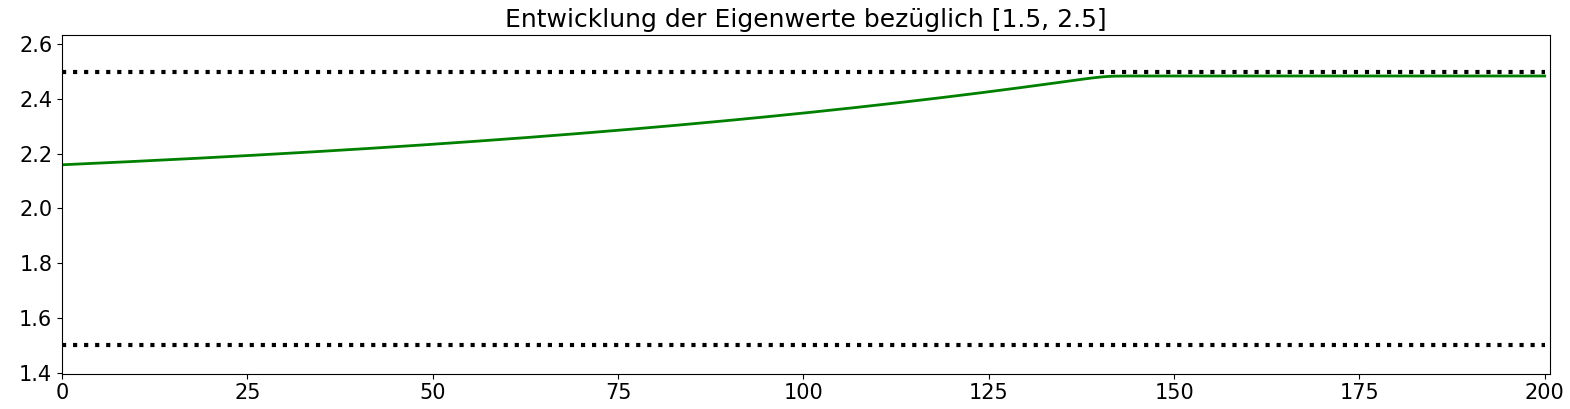
\includegraphics[width=0.9\textwidth, keepaspectratio]{./Original/Plot_1_100_0.05.png}
                  \caption{Plot zu System 1, $m=100$, $\lam_*=0.05$}
                  \label{fig: Plot_1_100_0.05}
            \end{figure}

            \begin{figure}[ht]
                  \centering
                  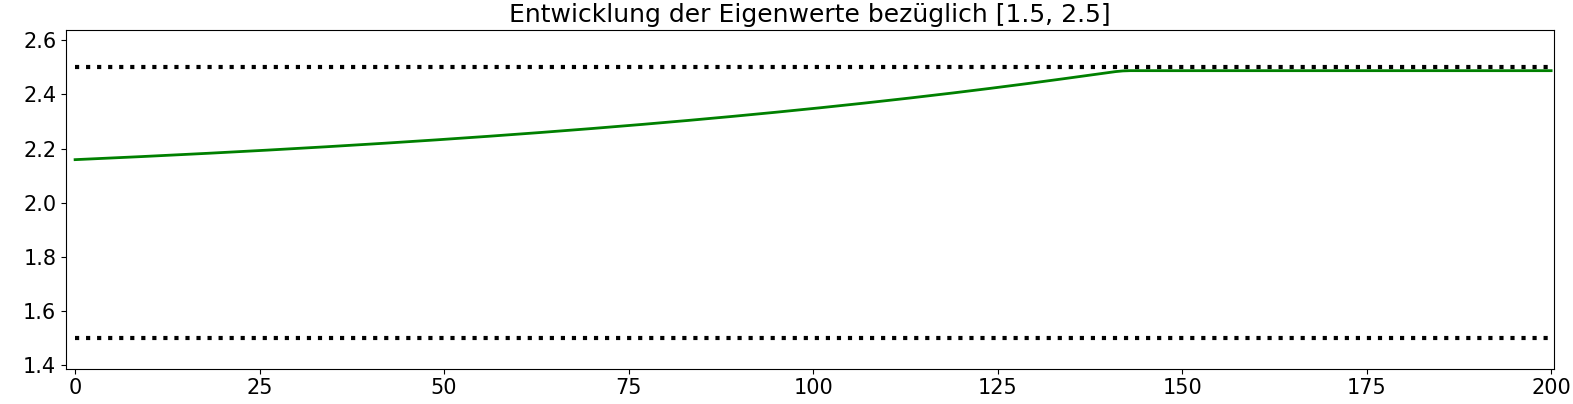
\includegraphics[width=0.9\textwidth, keepaspectratio]{./Original/Plot_1_150_0.05.png}
                  \caption{Plot zu System 1, $m=150$, $\lam_*=0.05$}
                  \label{fig: Plot_1_150_0.05}
            \end{figure}

            Man sehe zuerst, dass sich Eigenwert 2 dem oberen Rand des Intervalls nähert, aber ihn nicht überschreitet.
            Daran ändert sich auch nach weiteren 9800 Schritten nichts, wie man in Tabelle \ref{tab: Ergebnisse} erkennen kann.
            Die Unterschiede zwischen diesen Durchläufen kann man an den Verläufen der Eigenwerte 3-8 erkennen.
            Da diese Eigenwerte aber nicht im Intervall liegen, unterscheiden sich die Eigenwert-Zählungen dieser Durchläufe nicht sichtbar.
            Diese Tatsache kann man durch Ausführen des Programmes selber belegen.

            Bei den nächsten beiden Durchläufen betrachte nur die Schritte 0 bis 19. 

            \begin{figure}[ht]
                  \centering
                  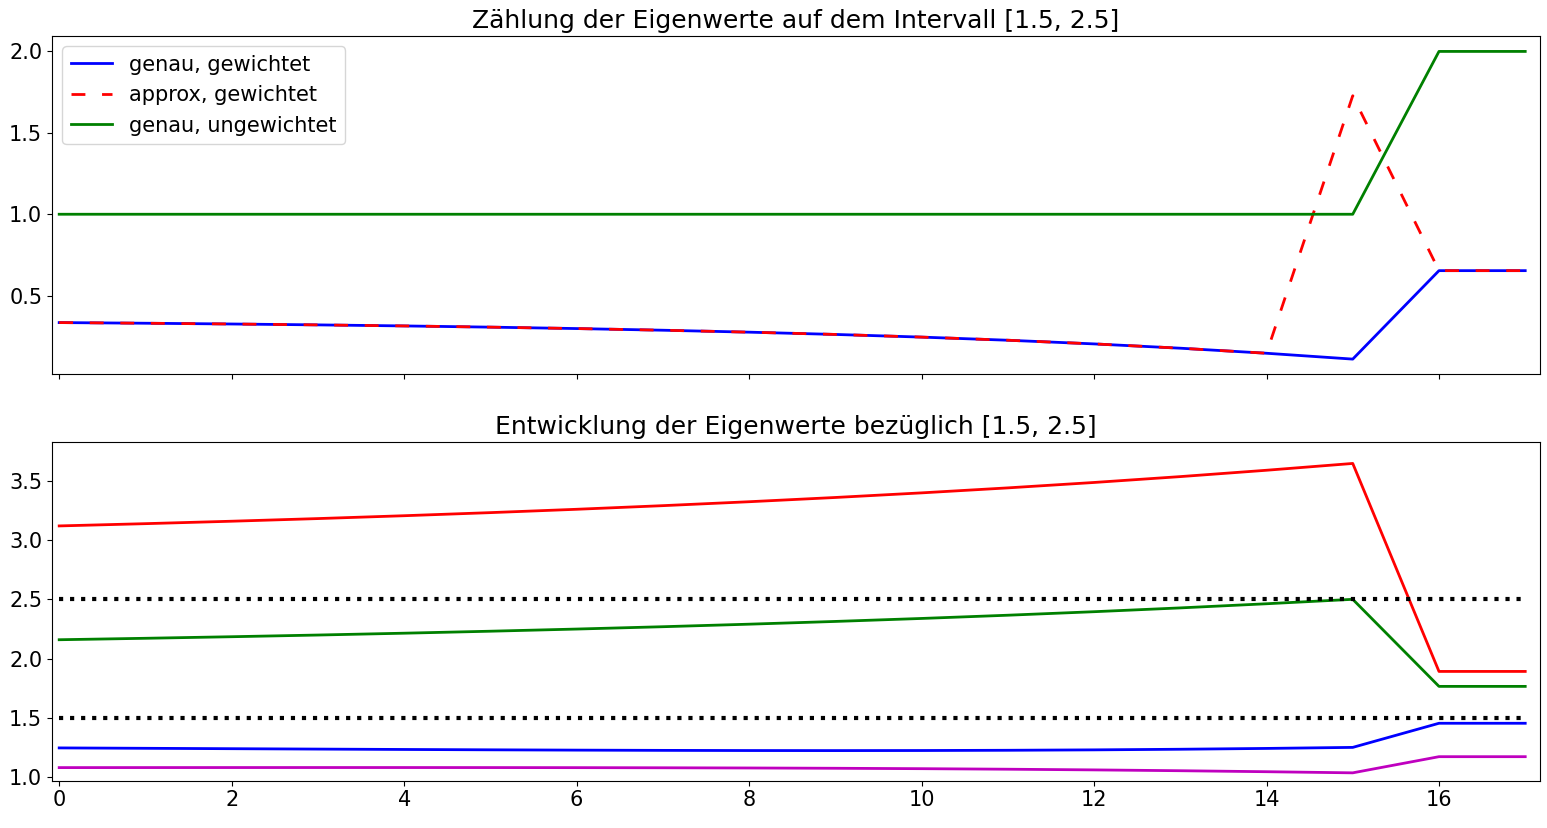
\includegraphics[width=0.9\textwidth, keepaspectratio]{./Original/Plot_1_100_0.5.png}
                  \caption{Plots zu System 1, $m=100$, $\lam_*=0.5$}
                  \label{fig: Plot_1_100_0.5}
            \end{figure}

            \begin{figure}[ht]
                  \centering
                  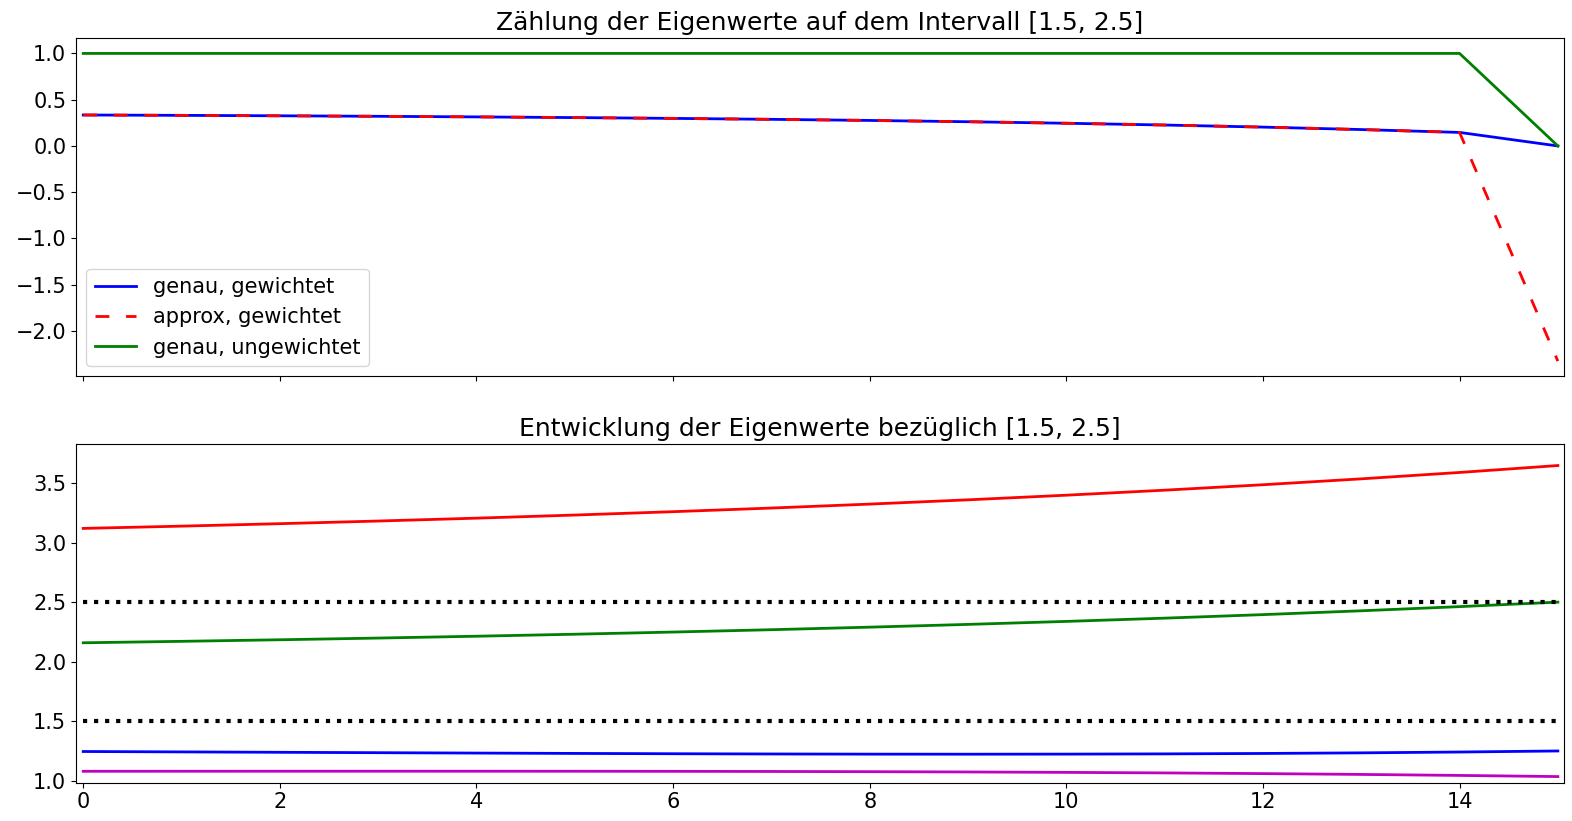
\includegraphics[width=0.9\textwidth, keepaspectratio]{./Original/Plot_1_150_0.5.png}
                  \caption{Plots zu System 1, $m=100$, $\lam_*=0.5$}
                  \label{fig: Plot_1_150_0.5}
            \end{figure}

            Hier kann man die Unterschiede zwischen den Genauigkeiten der Quadraturformeln erkennen: während in Abb. \ref{fig: Plot_1_100_0.5} nach Schritt 15 nicht alle Eigenwerte aus dem Intervall entfernt wurden,
            so wurde es in Abb. \ref{fig: Plot_1_150_0.5} vollbracht.

            Man sehe aber auch, dass die approximierte gewichtete Eigenwertzählung bei beiden Durchläufen sehr stark von der genauen abweicht.
            Dies kann sehr wahrscheinlich auf die verwendete Quadraturformel zurückgeführt werden:
            Bei beiden Quadraturformeln wird L(z,s) an den Stellen $z=\lambda_a$ und $z=\lambda_b$ ausgewertet.
            Falls aber ein Eigenwert sich nahe des Intervallrandes befindet, so sind diese Stützstellen nahe einer Polstelle.
            Das kann zu unvorhersagbaren Erscheinungen führen:
            Während in Abb. \ref{fig: Plot_1_100_0.5} bei Schritt 15 die gewichtete Eigenwertzählung viel zu hoch approximiert wird,
            so wird die approximierte gewichtete Eigenwertzählung in Abb. \ref{fig: Plot_1_150_0.5} bei Schritt 15 negativ.

            Bei Durchlauf \ref{fig: Plot_1_100_0.5} wird infolge dessen nun nicht mehr versucht, den zweiten Eigenwert zu vergrößern, damit er das obere Ende des Intervalls überschreitet, sondern er wird verringert, wodurch nun sogar der erste Eigenwert im Intervall liegt.
            Obwohl die negative Approximation bei Abb. \ref{fig: Plot_1_150_0.5} einen Wert annimmt, der für die genauen Eigenwertzählung nicht möglich ist, so ändert es nichts an dem Verlauf, da in diesem Schritt alle Eigenwert außerhalb des Intervalls liegen und laut Algorithmus \ref{alg: steilster Abstieg} die genaue gewichtete Zählung verwendet wird, um zu entscheiden, ob ein Minimum erreicht wurde.
            Sollte man nur Informationen über die approximierte Zählung besitzen, so wäre das Verfahren, je nach Programmierung, nicht beendet worden, sondern fortgeführt worden, obwohl es ein Minimum erreicht hatte.

            Dieses Verhalten der approximierten gewichteten Eigenwertzählung wird in Kapitel \ref{sec: Verbesserungen} erneut angesprochen.

            Betrachte nun die letzten zwei Durchläufe:
            Es wurde sich hier auf die Schritte 50-150 beschränkt, um diese im Detail sehen zu können.

            \begin{figure}[ht]
                  \centering
                  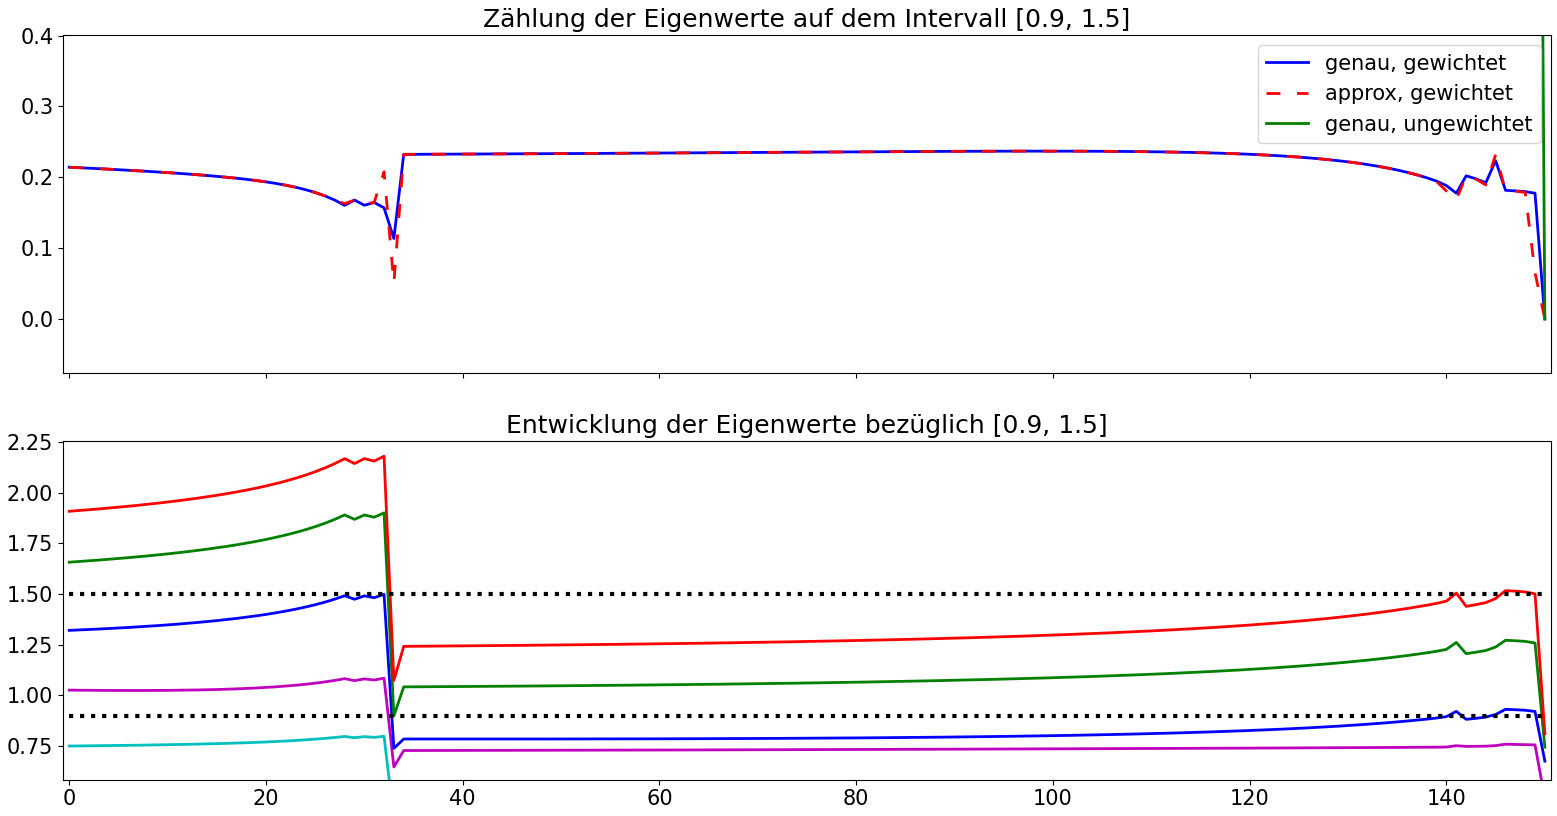
\includegraphics[width=0.9\textwidth, keepaspectratio]{./Original/Plot_2_100_0.05.png}
                  \caption{Plots zu System 2, $m=100$, $\lam_*=0.05$}
                  \label{fig: Plot_2_100_0.05}
            \end{figure}

            \begin{figure}[ht]
                  \centering
                  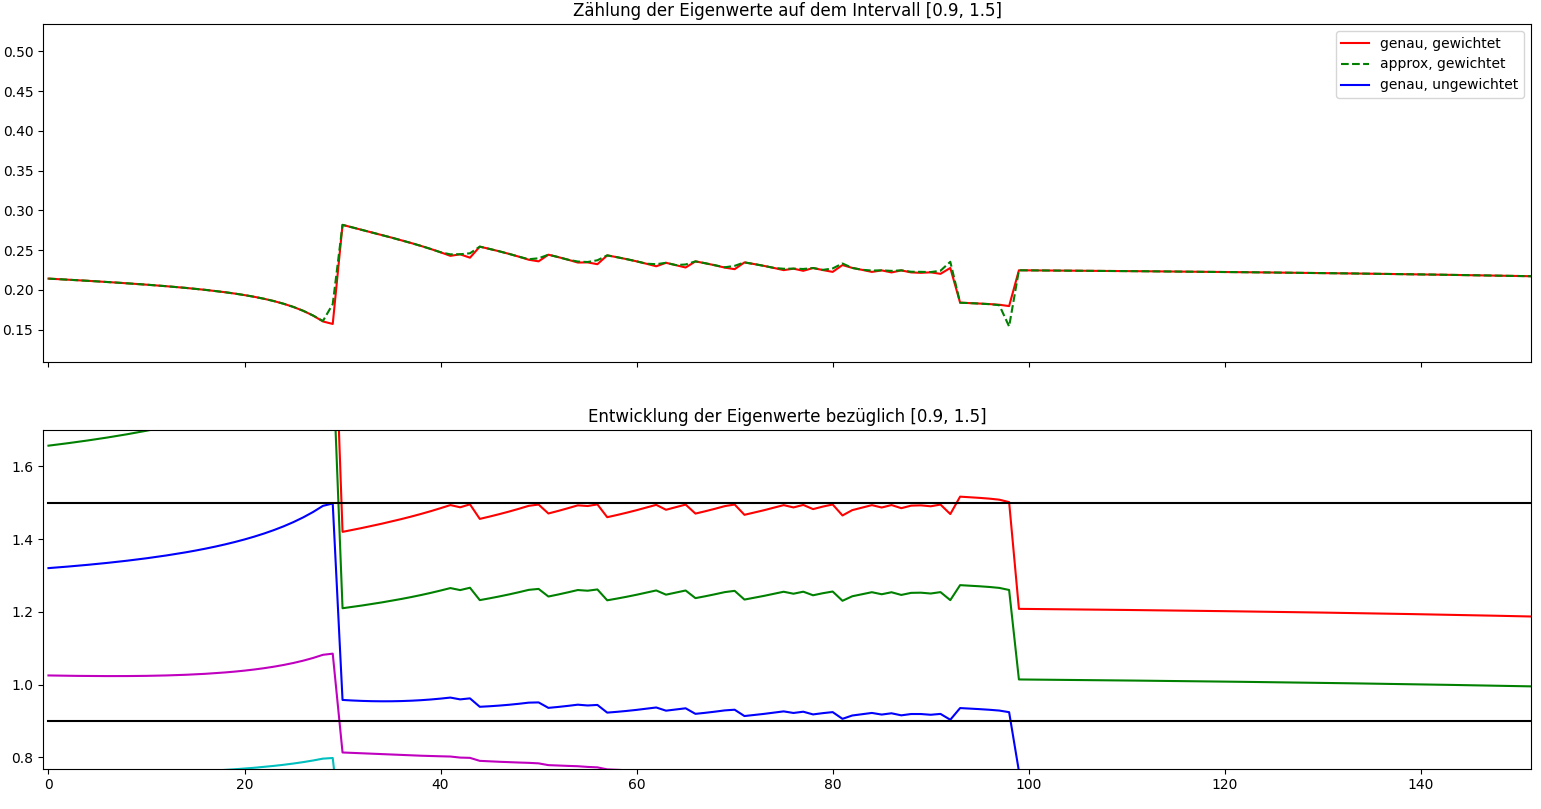
\includegraphics[width=0.9\textwidth, keepaspectratio]{./Original/Plot_2_150_0.05.png}
                  \caption{Plots zu System 2, $m=150$, $\lam_*=0.05$}
                  \label{fig: Plot_2_150_0.05}
            \end{figure}

            Hier sieht man, dass das Erreichen eines Minimums in Abb. \ref{fig: Plot_2_100_0.05} keine kontrollierte Veränderung von $s$ war, um einen einzelnen Eigenwert zu vergrößern/ verringern, sondern die Eigenwerte sich fast zufällig veränderten.
            Bei Abb. \ref{fig: Plot_2_100_0.05} traf der Algorithmus bei Schritt 150 nur zufällig einen Design-Parameter, durch welchen alle Eigenwerte außerhalb des Intervalls lagen.
            Durch die genauere Quadraturformel, die in Abb. \ref{fig: Plot_2_150_0.05} verwendet wurde, wurde $\nabla J^*(s)$ derart verändert, dass der letzte Design-Parametern aus Abb. \ref{fig: Plot_2_100_0.05} nicht erreicht wurde.
            Man kann hier die Suche nach einem passenden Parameter $s$ als fast chaotisches System betrachten, da eine Veränderung der genutzen Quadraturformel ausreicht, um den Verlauf der Minimierung komplett zu verändern\footnote{es reicht sogar ein Wechsel des Gerätes, welches das Programm ausführt, um unterschiedliche Ergebnisse hervorzubringen}.

\chapter{Verbesserungen}
\label{sec: Verbesserungen}
      In Kapitel \ref{sec: Programmieren} sind folgende Probleme deutlich zum Vorschein getreten:
      Einerseits ist die approximierte Zählung der Eigenwerte unzureichend, wenn sich ein Eigenwert in der Nähe der Intervallgrenzen befindet.
      Am einfachsten ist dies an den Abbildungen \ref{fig: Plot_1_100_0.5} und \ref{fig: Plot_2_100_0.05} zu sehen:
      Immer wenn ein Eigenwert in die Nähe der Intervallgrenze und damit der Integrationskurve kam, wurde die gewichtete Eigenwertzählung ungenau approximiert, was dazu führte, dass die Systeme in einem Schritt sehr große Sprünge ausführten.
      Auch das Verhalten des Eigenwerts in den Abbildungen \ref{fig: Plot_1_100_0.05} und \ref{fig: Plot_1_150_0.05} kann damit erklärt werden. Hier kam es zwar nicht zu Sprüngen, aber wahrscheinlich verhinderte diese Quadraturformel, dass der Parameter so verändert wird, dass der Eigenwert das Intervall verlassen kann.
      Ferner sieht man anhand der Abbildungen \ref{fig: Plot_1_100_0.05}, \ref{fig: Plot_1_150_0.05} und \ref{fig: Plot_1_150_0.5}, dass eine größere Schrittweite des Gradientenverfahrens deutlich bessere Ergebnisse hervorbringen kann.
      Allerdings ist eine zu hohe Schrittweite nicht immer von Vorteil, sollte sich ein Schritt des Verfahrens nahe an einer Lösung des Problems befinden.
      Man sehe zudem, dass sich viele der Durchläufe über lange Strecken kaum verändern.
      Zuletzt sind diese langen Zeiten für Probleme mit einstelligen Freiheitsgraden nicht wünschenswert, da einige Systeme $n>1.000.000$ Freiheitsgrade einbeziehen (vgl. \cite[S. 359]{maschinendynamikDresig}).

      \section{Verbesserte Quadraturformeln}
            Man wende sich zuerst der Verbesserung der Quadraturformel zu.
            Dadurch erhofft man sich, großen Sprünge in der Verteilung der Eigenwerte zu vermeiden, um zu gewährleisten, dass die Eigenwerte geordnet das Intervall verlassen und nicht per Zufall wie in Abb. \ref{fig: Plot_2_100_0.05}.

            Man nutze daher eine Quadraturformel, welche das Integral zwar approximiert, aber nicht an den Stellen $\lambda_a$ und $\lam_b$ ausgewertet wird.

            Die einfachste Quadraturformel, die dies bewerkstelligt ist die \zitat{Mittelpunkts-Regel}\cite[S. 526]{numerikHermann}:

            Sei dazu $\gamma_k, k=0,\dots,m-1$ wie in (\ref{def: gamma_k}). Nach (\ref{eqn: Teilintegral Kurve zu Intergral normal}) gilt:
            \begin{align*}
                  \int_{\gamma_k} L(z, s)\ dz =& \int_{2\pi \frac{k}{m}}^{2\pi\frac{k+1}{m}}L(\Tilde z_0+\Tilde r\exp(it), s)i\Tilde r \exp(it)\ dt\\
                  \approx& L(\Tilde z_0+\Tilde r\exp\klammer{\frac{2\pi i}{m}(k+\frac{1}{2})}, s)i\Tilde r \klammer{\frac{2\pi i}{m}(k+\frac{1}{2})} \frac{2\pi}{m}\\
                  =& L(z_{k+\frac{1}{2}}, s)(\Tilde z_0-z_{k+\frac{1}{2}}) \frac{2\pi i}{m}
            \end{align*}

            wobei die Definition $z_{k+\frac{1}{2}}:= \Tilde z_0+\Tilde r\exp(\frac{2\pi i}{m}(k+\frac{1}{2})), k=0,\dots,m$ und die Formel für die Mittelpunkts-Regel aus \cite[S. 526]{numerikHermann} verwendet wurde.

            Es gilt für $J(s)$:
            \begin{align}
                  J(s) =& \frac{1}{2\pi i}\sum_{k=0}^{m-1} \int_{\gamma_k} L(z, s)\ dz = \frac{1}{2\pi i}\sum_{k=0}^{m-1} L(z_{k+\frac{1}{2}}, s)(\Tilde z_0-z_{k+\frac{1}{2}}) \frac{2\pi i}{m}\nonumber\\
                  =&  \frac{1}{2\pi i}\left[\frac{2\pi i}{m}\sum_{k=0}^{m-1} L(z_{k+\frac{1}{2}}, s)(\Tilde z_0-z_{k+\frac{1}{2}})\right]\label{def: Mittelpunkts-Regel, angewendet}
            \end{align}

            Wobei wieder die Faktoren vor der Summe nicht gekürzt wurden, da der erste Faktor von der Anwendung des Residuensatzes stammt und der zweite Faktor ein Teil der Quadraturformel ist\footnote{falls man die Faktoren kürzt, erhält man die Stützstellen $z_k$ und Gewichte $\w_k$ aus \cite[S. 128]{grundlageFutamura}}.

            Durch die Verwendung dieser Quadraturformel erhält man folgende Ergebnisse:

            \begin{table}[!ht]
                  \centering
                  \begin{tabular}{lllcc}
                       System & $m$ & $\lambda_*$ & Iterationen & Zeit in s\\
                       \hline
                       1 & $100$ & $0.05$ & $142$ & $3.7$ \\ 
                       1 & $150$ & $0.05$ & $143$ & $5.3$ \\
                       \hline
                       1 & $100$ & $0.5$ & $15$ & $0.5$ \\
                       1 & $150$ & $0.5$ & $15$ & $0.7$ \\
                       \hline
                       2 & $100$ & $0.05$ & $300$ & $13.9$ \\
                       2 & $150$ & $0.05$ & $289$ & $21.7$ \\
                       \hline
                  \end{tabular}\\
                  \captionof{table}{Kennzahlen bei Verwendung der Mittelpunkts-Regel}\label{tab: Ergebnisse_Mittelpunkt}
            \end{table}

            Die Ergebnisse und die zugehörigen Plots können auch in der Datei \textit{./Programmierung/Verbesserung\_Mittelpunkt.py} betrachtet werden.

            Wie man sehen kann, erfolgen die Berechnungen der ersten zwei Durchläufe nun viel schneller, da nur 142-143 Schritte benötigt werden.
            Man beachte auch, dass hier in den Durchläufen zu System 1 die Anzahl an benötigten Iterationen um den Faktor dividiert wird, um welchen die Schrittweite $\lam_*$ multipliziert wird, was auf die Eindimensionalität von Design-Parameter $s$ zurückzuführen ist.
            In den Durchläufen zu System 2 sieht man zudem, dass sich die Anzahl an Iterationen für $m=100$ im Vergleich zu Tabelle \ref{tab: Ergebnisse} verdoppelt, allerdings ist dies auf die Tatsache zurückzuführen, dass der Verlauf der Eigenwerte keine plötzlichen Sprünge mehr ausführt, wie sie in Abb. \ref{fig: Plot_2_100_0.05} zu sehen waren.

            \begin{figure}[ht]
                  \centering
                  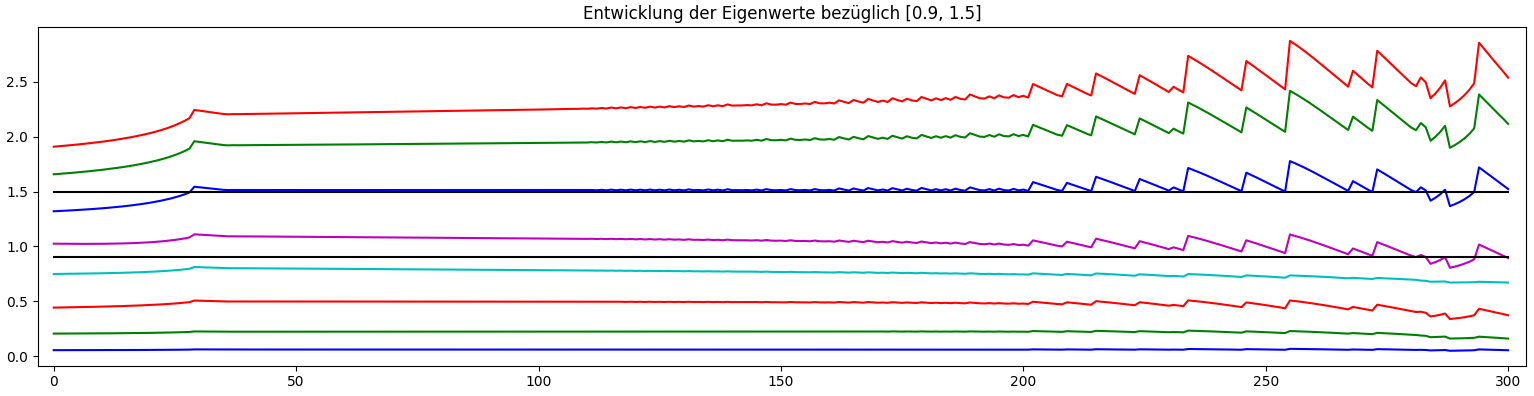
\includegraphics[width=0.9\textwidth, keepaspectratio]{./Verbesserung_Mittelpunkt/Plot_2_100_0.05.png}
                  \caption{Plot zu System 2, $m=100$, $\lam_*=0.05$, Mittelpunkts-Regel verwendet}
                  \label{fig: Plot_2_Mittelpunkt}
            \end{figure}

            Natürlich wären diese Durchläufe auch schneller, wenn sie kein Ergebnis bringen, da hier die Funktion nur an einer Stelle auszuwerten ist.

            Nehme daher als zweites Beispiel die \zitat{Zweipunkt-Formel}\cite[S. 526]{numerikHermann}. Analog zu (\ref{def: JStern}) und (\ref{def: Mittelpunkts-Regel, angewendet}) folgt:
            \begin{align}
                  J(s) = \frac 1 {2\pi i}\left[\frac{\pi i \Tilde r}{m}\sum_{k=0}^{m-1}\klammer{L(z_{k,-}, s)\exp\klammer{-\frac{\pi i}{\sqrt{3}m}}+L(z_{k,+}, s)\exp\klammer{\frac{\pi i}{\sqrt{3}m}}}\right]
            \end{align}
            mit $z_{k,\pm}:=\Tilde z_0+\Tilde r\exp\klammer{\frac{\pi I}{\sqrt{3}m}(2\sqrt 3 k+\sqrt 3 \pm 1)}$

            Diese Formel erhält man durch Anwenden der Zweipunkt-Formel aus \cite[S. 526]{numerikHermann} mit $u= \frac{2\pi}{m}(k+\frac 1 2)$ und $v=\frac \pi m$.

            Es folgen die Ergebnisse des Programms \textit{./Programmierung/Verbesserung\_Gauss2.py}.

            \begin{table}[!ht]
                  \centering
                  \begin{tabular}{lllcc}
                       System & $m$ & $\lambda_*$ & Iterationen & Zeit in s\\
                       \hline
                       1 & $100$ & $0.05$ & $145$ & $7.5$ \\ 
                       1 & $150$ & $0.05$ & $145$ & $10.3$ \\
                       \hline
                       1 & $100$ & $0.5$ & $15$ & $0.9$ \\
                       1 & $150$ & $0.5$ & $15$ & $1.1$ \\
                       \hline
                       2 & $100$ & $0.05$ & $112$ & $11.9$ \\
                       2 & $150$ & $0.05$ & $63$ & $9.3$ \\
                       \hline
                  \end{tabular}\\
                  \captionof{table}{Kennzahlen bei Verwendung der Zweipunkt-Formel}\label{tab: Ergebnisse_Gauss2}
            \end{table}

            Obwohl die Zweipunkt-Formel eine \zitat{Gaußsche Quadraturformel}\cite[S. 523]{numerikHermann} ist und damit einen optimalen Genauigkeitsgrad von 5 besitzt (vgl. \cite[S. 522f.]{numerikHermann}), so ist der Unterschied zur Mittelpunkts-Regel in den Durchläufen zu System 1 gering.
            In den letzten beiden Plots kann aber festgestellt werden, dass sich die Anzahl an benötigten Iteration stark verringert.

            \begin{figure}[ht]
                  \centering
                  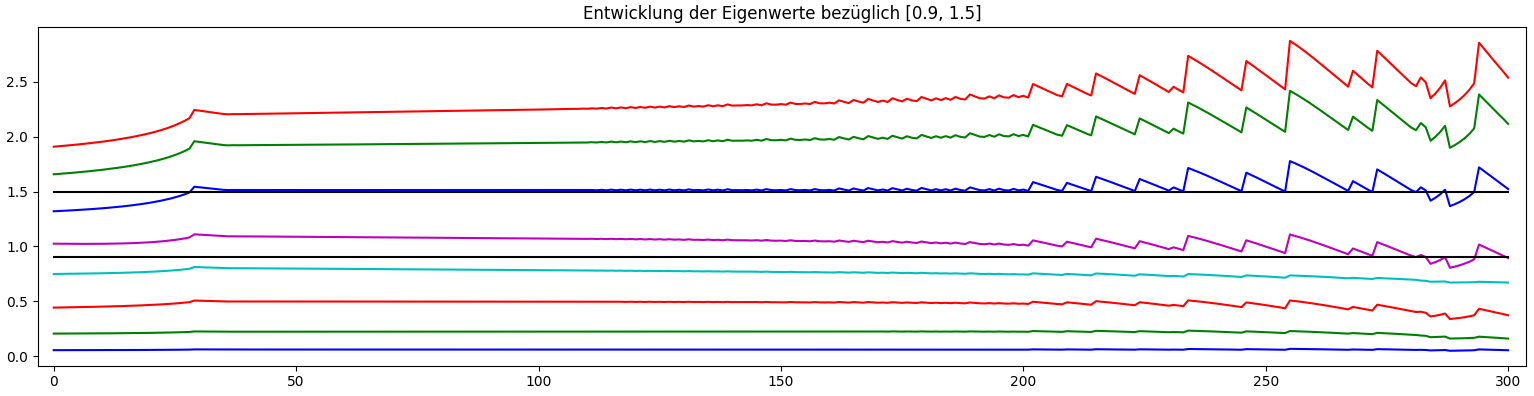
\includegraphics[width=0.9\textwidth, keepaspectratio]{./Verbesserung_Mittelpunkt/Plot_2_100_0.05.png}
                  \caption{Plot zu System 2,$m=100$, $\lam_*=0.05$, Zweipunkt-Formel verwendet}
                  \label{fig: Plot_2_150_0.05_Gauss2}
            \end{figure}

            Ferner sehe man in Abb. \ref{fig: Plot_2_150_0.05_Gauss2}, dass sich die Eigenwerte nun nicht mehr wiederholen, wie es in Abb. \ref{fig: Plot_2_Mittelpunkt} der Fall war.
            Man nehme daher für die Minmierung der Eigenwerte in dem restlichen Kapitel immer die Zweipunkt-Formel.

            Die Tatsache, dass diese zwei Quadraturformeln nicht bei $\lam_a$ und $\lam_b$ ausgewertet werden und sie deshalb besser sind, kann man auch an Programm
            \textit{./Programmierung/Vergleich Quadraturformeln.py} sehen. Dort wurde noch die verschobene Trapezregel angewendet, welche die Stütztellen $z_{k+\frac 1 2}$ statt $z_k$ verwendet.
            Allein dies macht einen gewaltigen Unterschied:

            Für eine immer näher an $\lambda_b = 1$ rückende Polstelle wächst die Trapezformel aus (\ref{def: JStern}) sehr stark an. Alle anderen Quadraturformeln nähern sich stattdessen $0.5$.
            Wie auch in den Durchläufen zu System 1 liegen die Ergebnisse der Mittelpunkts-Regel und der Zweipunkt-Formel sehr dicht beieinander.
            Wie man aber auch sehen kann, ist die höhere Genauigkeit bei System 2 nun von großer Bedeutung:
            Die Durchläufe mit der Zweipunkt-Formel benötigen viel weniger Iterationen und sind daher schneller.
            Ferner kommt dazu, dass nun auch die Wahl von $m$ eine Rolle spielt: in den Tabellen \ref{tab: Ergebnisse_Mittelpunkt} und \ref{tab: Ergebnisse_Gauss2} verringert sich die Anzahl an Iterationen bei erhöhter Anzahl an Stützstellen.
            Aufgrund des damit verbundenen erhöhten Rechenaufwands benötigt der letzte Durchlauf aus Tabelle \ref{tab: Ergebnisse_Mittelpunkt} aber noch mehr Zeit als der vorletzte.
            Bei der Zweipunkt-Formel wurden aber so viele Schritte eingespart, dass nun der letzte Durchlauf weniger Zeit beansprucht als der Durchlauf mit $m=100$.

            Verwende daher ab nun immer die Zweipunkt-Formel, um zu einem bestmöglichen Ergebnis zu kommen.

      \section{dynamische Schrittweite}
            Als nächstes wende man sich dem Gradientenverfahren zu:
            Die Schrittweite $\lambda_*$ soll nun nicht mehr fest sein, sondern möglichst optimal berechnet werden.

            Werte daher nablaJ\_Stern an den Stellen $x-d*t, t=\lambda_*\N$ an\footnote{obwohl $\lambda_*$ nicht mehr direkt die Schrittweite bestimmt, so benötigt man trotzdem eine Schrittweite, wie weit die berechneten Stellen auseinander liegen sollen}.

            Der Algorithmus zur Bestimmung des neuen Punktes ist wie folgt definiert:
            \begin{algorithm}
                  \caption{Bestimmung des nächsten Punktes}
                  \label{alg: dynamischerPunkt}

                  \begin{algorithmic}
                        \Require $\nabla J(s), s, d, \lambda_*, \Omega$
                        \Ensure $s^*$
                        \State $s_{\text{alt}} = s;$
                        \For {$i = 1,\dots,1000$}\Comment{stellt sicher, dass Schleife nicht unendlich läuft}
                              \State $s_{\text{neu}} = s_{\text{alt}}-\lambda_* d$;
                              \If{$s_{\text{neu}}\notin \Omega$}
                                    \State\Return $s_{\text{neu}}$;
                              \ElsIf{$|\nabla J(s_{\text{neu}})\cdot d^T| < 0.00001$}
                                    \State\Return $s_{\text{neu}}$;
                              \ElsIf{$\nabla J(s_{\text{neu}})\cdot d^T < 0$}
                                    \If{$i=1$}
                                          \State\Return $s_{\text{neu}}$;
                                    \Else
                                          \State\Return $s_{\text{alt}}$;
                                    \EndIf
                              \EndIf
                              \State $s_{\text{alt}} = s_{\text{neu}}$;
                        \EndFor
                  \State\Return $s_{\text{neu}};$
                  \end{algorithmic}
            \end{algorithm}

            Hierbei ist $s$ der alte Wert, $d$ die approximierte Ableitung an diesem Wert, $\lam_*$ die Schrittweite und $\Omega$ der zulässige Bereich des Design-Parameters $s$.
            Diese Funktion gibt einen Wert s aus, der möglichst nahe an der optimalen Stelle ist.
            An dieser Stelle würde laut \cite[S. 286]{optimierungBurkhard}
            $$\nabla J(s)\cdot d^T = 0$$ gelten, da die Ableitung aber nur approximiert wurde, reiche hier 


            Das Anwenden dieses Algorithmus zur Bestimmung des nächsten Punktes bringt folgende Ergebnisse:
            \begin{table}[!ht]
                  \centering
                  \begin{tabular}{lllcc}
                       System & $m$ & $\lambda_*$ & Iterationen & Zeit in s\\
                       \hline
                       1 & $100$ & $0.05$ & $1$ & $10.4$ \\ 
                       1 & $150$ & $0.05$ & $1$ & $17.26$ \\
                       \hline
                       1 & $100$ & $0.5$ & $1$ & $1.8$ \\
                       1 & $150$ & $0.5$ & $1$ & $3.1$ \\
                       \hline
                       2 & $100$ & $0.05$ & $24$ & $16.7$ \\
                       2 & $150$ & $0.05$ & $178$ & $62.0$ \\
                       \hline
                  \end{tabular}\\
                  \captionof{table}{Kennzahlen bei Verwendung eines dynamischen Schrittweite}\label{tab: Ergebnisse_dynamischSchritt}
            \end{table}

            Die Ergebnisse sind auch in \textit{./Programmierung/Verbesserung\_dynamischeSchrittweite.py} zu finden.

            Wie man sehen kann, wird die Eigenwertzählung bei System 1 innerhalb eines Schrittes minimiert.
            Dies war aber zu erwarten, da $s$ in System 1 ein Skalar war.
            Sofern die Ableitung hier immer in das gleiche Vorzeichen, gehen auch alle anderen Durchläufe aus Kapitel \ref{sec: Verbesserungen} bei System 1 immer nur in eine Richtung.
            Somit macht hier das Verfahren in einem Schritt, was vorher in $n$ Schritten gemacht wurde.

            Der Algorithmus kann aber auch hinderlich sein, wie man in Abb. \ref{fig: Plot_2_150_0.05_dynamischSchritt} sehen kann.
            \begin{figure}[ht]
                  \centering
                  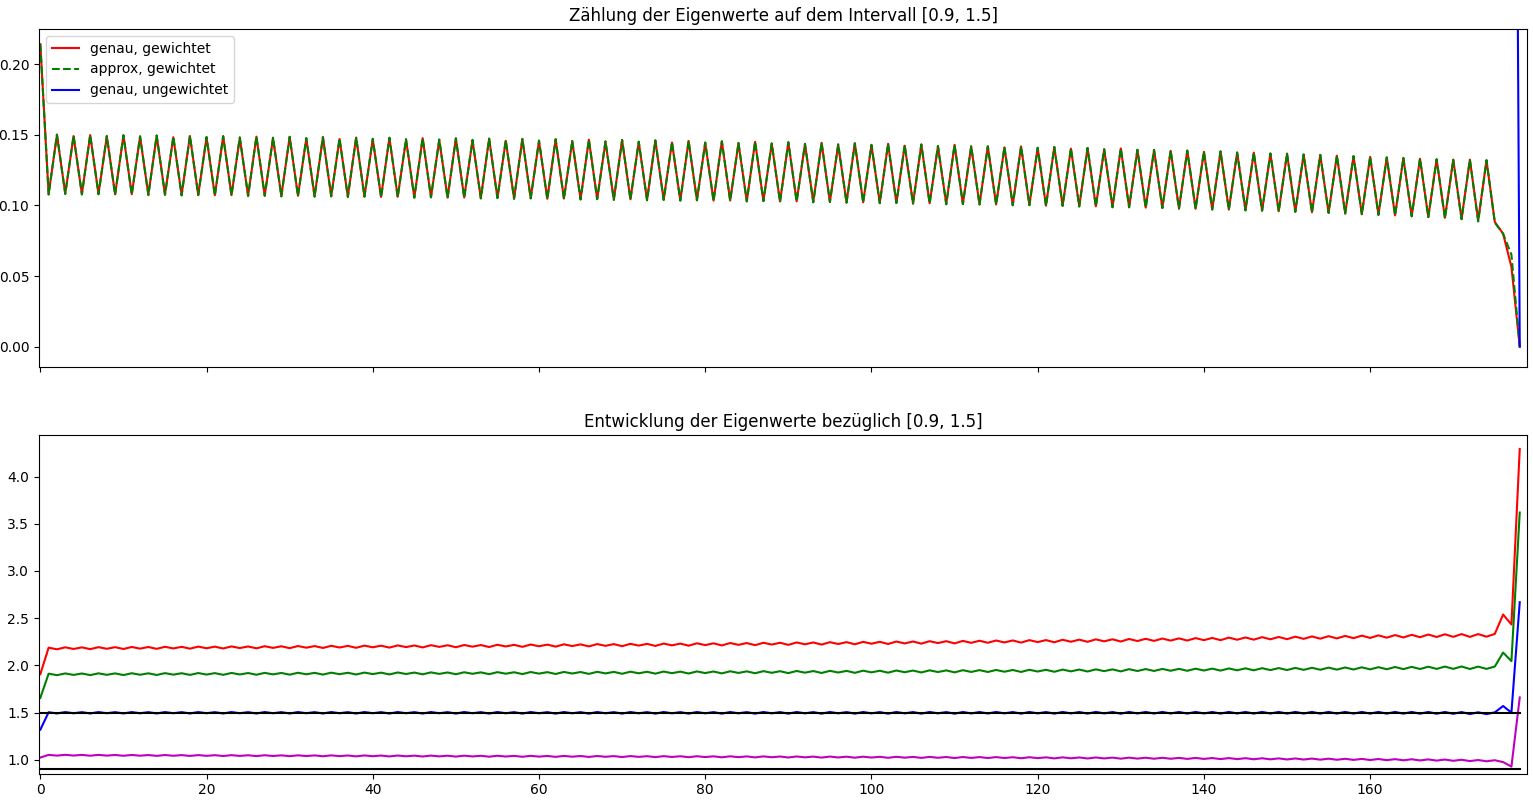
\includegraphics[width=0.9\textwidth, keepaspectratio]{./Verbesserung_dynamischeSchrittweite/Plot_2_150_0.05.png}
                  \caption{Plots zu System 2, $m=150$, $\lam_*=0.05$ bei Verwendung einer dynamischen Schrittweite}
                  \label{fig: Plot_2_150_0.05_dynamischSchritt}
            \end{figure}

            Hier verändert sich die Verteilung der Eigenwert und auch die Eigenwertzählungen nur sehr langsam.

      \section{Approximation von der Ableitung von J durch ein Differenzenverfahren}

            Zuletzt bemerke zuerst, dass die Approximation des Integrals durch die Quadraturformel die meiste Zeit benötigt, hingegen die genaue gewichtete Eigenwertzählung $J(s)$ sehr schnell berechnet werden kann.
            Da aber keine explizite Abhängigkeit vom Design-Parameter $s$ besteht, ist diese Formel nur gut, um als Abbruchbedingung des Gradientenverfahrens zu dienen.

            Approximiere man aber $\nabla J$ durch die Anwendung eines Differenzenverfahren auf $J(s)$ aus (\ref{def: J original}), wie es in Kapitel \ref{sec: Programmieren}angewendet wurde, um $\frac {dM}{ds}$ zu approximieren,
            so kann man diese Funktion nutzen, um die Berechnung von $\nabla J^*(s)$ und damit die Anwendung der Quadraturformel zu umgehen\footnote{man ersetzt also die Ableitung der Approximation von $J$ durch die Approximation der Ableitung von $J$}.

            Da diese Berechnung sehr viel schneller ist, erhöhe die maximal mögliche Anzahl an Iterationen pro Durchlauf auf 100000.
            Die Anzahl an Teilintervallen wird zwar nicht für die Berechnung an sich benötigt, aber die aufgerufene Funktion gibt für jeden Wert des Design-Parameters $s$ auch ein entsprechendes $J^*(s)$ zurück, um die Plots zu erstellen.
            Um diesen Mehraufwand so gering wie möglich zu halten sei $m=1$. Die approximierte gewichtete Eigenwertzählung wird dadurch zwar sehr ungenau, aber hier wird sie für keinen Schritt des Gradientenverfahrens verwendet.
            Die folgenden Ergebnisse können in \textit{./Programmierung/Verbesserung\_NablaJ.py} wiedergefunden werden.

            \begin{table}[!ht]
                  \centering
                  \begin{tabular}{lllcc}
                       System & $m$ & $\lambda_*$ & Iterationen & Zeit in s\\
                       \hline
                       1 & $1$ & $0.05$ & $31$ & $0.02$ \\ 
                       \hline
                       1 & $1$ & $0.5$ & $4$ & $0.0$ \\
                       \hline
                       2 & $1$ & $0.05$ & $>100000$ & $>198$ \\
                       2 & $1$ & $0.05$ & $>150000$ & $>428$ \\
                       2 & $1$ & $0.05$ & $>300000$ & $>1233$ \\
                       \hline
                  \end{tabular}\\
                  \captionof{table}{Kennzahlen bei Verwendung von $\nabla J(s)$}\label{tab: Ergebnisse_nablaJ}
            \end{table}

            Man beachte, dass diese Approximation für System 1 genau genug war, um ein Minimum innerhalb von 0.02 s zu finden.
            Allerdings ist dieses Verfahren in dieser Form für System 2 unzureichend. Man könnte die Ableitung genauer approximieren, indem die Schrittweite $h$ aus (\ref{def: DiffVerfahren}) verringert.
            Ferner würde vielleicht eine größere Schrittweite $\lambda_*$ helfen.

            Für die Durchläufe für System 2 erkenne man auch, dass die Zeit nun nicht mehr proportional zu den gegangenen Schritten ist.
            Dies liegt wahrscheinlich daran, dass nicht mehr alle Werte im Arbeitsspeicher gespeichert werden konnten, wodurch die Zugriffszeiten sich verlängerten.

            Da solche Überlegungen aber auch bei den anderen Varianten nicht implementiert wurden, werden sie hier auch nicht betrachtet.
\chapter{Auswertung}
\label{sec: Auswertung}

      In dieser Arbeit wurden in Kapitel \ref{sec: EW Problem_Futamura} der Matrix-Pencil, die Eigenwerte eines Matrix-Pencils, die allgemeine Schur-Zerlegung und die Identität von Futamura vorgestellt.
      Während die Schur-Zerlegung für den Beweis der Identität von Futamura benötigt wird, liefert sie auch eine Aussage über die Eigenwerte des Matrix-Pencils.
      Diese Identität erlaubt eine direkte Aussage über die Anzahl an Eigenwerten in einem Intervall, dafür muss aber ein Kurvenintegral berechnet werden.

      In Kapitel \ref{sec: MS Matrizen} wurden die Systeme vorgestellt, welche in Kapitel \ref{sec: Programmieren} und \ref{sec: Verbesserungen} behandelt werden.
      Um die Eigenwerte dieser Systeme zu berechnen, wurden die Massen- und Steifigkeitsmatrizen der Systeme berechnet und eine Formel für die Berechnung der Eigenkreisfrequenzen aufgestellt.
      Durch eine Substitution in dieser Formel erhält man in () die Formel für die Eigenwerte des Matrix-Pencils $(K-\lambda M)$.

      In Kapitel \ref{sec: EW Zählung} wurde die gewichtete Eigenwertzählung auf einem Intervall hergeleitet. Diese Funktion besitzt die Form aus (\ref{def: J original}) und ist einfach zu berechnen, hängt aber nicht direkt von dem Design-Parameter $s$ ab,
      wodurch sie nicht so einfach für ein Minimierungsverfahren verwendet werden kann.

      Durch die Identität von Futamura, dem Residuensatz und einer Quadraturformel erhält man in (\ref{def: JStern}) eine Approximation dieser Eigenwertzählung, welche direkt von $s$ abhängt.

      Diese Approximation wird in Kapitel \ref{sec: Programmieren} genutzt, um die Eigenwerte der Systeme auf einem Intervall zu zählen und anschließend zu eliminieren.
      
      Als Quadraturformel wurde hier die normale Trapezformel verwendet, welche aber unzureichende Ergebnisse brachte.

      Unter anderem wurde in Kapitel \ref{sec: Verbesserungen} diese Problem behoben.
      Während in Kapitel \ref{sec: Programmieren} die Schrittweite des Gradientenverfahrens noch fest war, so wurde in Kapitel \ref{sec: Verbesserungen} ein Algorithmus definiert, der den nächsten Wert von $s$ dynamisch bestimmt.
      Dieses Verfahren erlaubte es zwar die Eigenwerte des ersten Systems in einem Schritt aus dem gegebenen Intervall zu entfernen, aber es benötigt insgesamt mehr Zeit als ein analoges Gradientenverfahren mit fester Schrittweite.

      Zuletzt wurde in Kapitel \ref{sec: Verbesserungen} auch eine Approximation der Ableitung von $J(s)$ eingeführt. Diese kann zwar die Eigenwertzählung von System 1 unglaublich schnell minimieren, sie versagte aber bei einem mehrdimensionalen Design-Parameter, wie er in System 2 genutzt wird.

      Der schnellste Weg zur Minimierung der Eigenwertzählung ist daher eine möglichst genaue Quadraturformel, welche möglichst wenig Stützstellen benötigt, um ein gutes Ergebnis mit geringstem Zeitaufwand zu erhalten.

      Damit sind offenbar die Gauss-Quadraturformeln gemeint.

\chapter{Literaturverzeichnis}

      \printbibliography
% es fehlt Bilderverzeichniss

%%
%% Erscheint auf letzter Seite
%%
\chapter*{Erkl\"{a}rung}
\thispagestyle{empty}
Hiermit erkl\"{a}re ich, dass ich die am \datum\ eingereichte Bachelorarbeit zum Thema
\emph{\thema} unter Betreuung von \betreuer\ selbstst\"{a}ndig erarbeitet,
verfasst und Zitate kenntlich gemacht habe. Andere als die angegebenen Hilfsmittel
wurden von mir nicht benutzt.

\bigskip \bigskip \bigskip \bigskip \bigskip

Dresden, \datum\ \hfill Unterschrift

\normalsize
\end{document}



